%%%%%%%%%%%%%%%%%%%%%%%%%%%%%%%%%%%
%%%  Filename: thesis_template.tex
%%%  ---
%%%  Template for Master Thesis at DTETI UGM   		
%%%  Created using thesisdtetiugm.cls
%%%  --- 
%%%  Written by Canggih Puspo Wibowo
%%%  [canggihpw@gmail.com]
%%%%%%%%%%%%%%%%%%%%%%%%%%%%%%%%%%%

%% Use option "bahasa" or "english" 
%%    to change the basic language used
%% User option "bachelor", "master", or "doctoral"
%% 	  to change the degree
% \documentclass[<bachelor/master/doctoral>,<bahasa/english>]{thesisdtetiugm}
\PassOptionsToPackage{table}{xcolor}
\documentclass[bachelor,bahasa]{thesisdtetiugm}
\usepackage{tabularx}
\newenvironment{conditions*}
  {\par\vspace{\abovedisplayskip}\noindent
   \tabularx{\columnwidth}{>{$}l<{$} @{${}={}$} >{\raggedright\arraybackslash}X}}
  {\endtabularx\par\vspace{\belowdisplayskip}}
%======================================
% Information Input
%======================================
% Input author's name and ID number
\author{Ade Firmansyah}{19/440303/TK/48630}
% Input the thesis' title
\title{Peningkatan Pendeteksian \emph{Copy Detection Pattern} pada \emph{Secure QR Code} Menggunakan Penanda ArUco}
% Program and the head of the program
\program{Teknologi Informasi}{<<Program coordinator>>}{<<NIP>>}
% Name of department head and NIP
\departmenthead{<<Head of the department>>}{<<NIP>>}
\major{<<Major>>}
\yearsubmit{2023}
\examdate{<<Exam date>>}
% Name of thesis supervisors/promotors
\addsupervisor{Syukron Abu Ishaq Alfarozi, S.T., Ph.D.}{NIKA 1111 9920 5202 10 1 102}
\addsupervisor{Azkario Rizky Pratama, S.T., M.Eng., Ph.D.}{NIKA 1111 9910 2201 60 7 102}
%\addsupervisor{<<Supervisor 3>>}{<<NIP>>}
% Name of examiners
%\addexaminer{<<Examiner 1>>}{<<NIP 1>>}
%\addexaminer{<<Examiner 2>>}{<<NIP 2>>}
%\addexaminer{<<Examiner 3>>}{<<NIP 3>>}
%\addexaminer{<<Examiner 4>>}{<<NIP 4>>}
%\addexaminer{<<Examiner 5>>}{<<NIP 5>>}
%\addexaminer{<<Examiner 6>>}{<<NIP 6>>}
%\addexaminer{<<Examiner 7>>}{<<NIP 7>>}
%\addexaminer{<<Examiner 8>>}{<<NIP 8>>}
%\addexaminer{<<Examiner 9>>}{<<NIP 9>>}

%======================================

% correct bad hyphenation here [example]
% \babelhyphenation[<<english/bahasa>>]{op-tical net-works semi-conduc-tor}
%% Uncomment block of code below to disable hyphenation
%\tolerance=1
%\emergencystretch=\maxdimen
%\hyphenpenalty=10000
%\hbadness=10000

\begin{document}
%======================================
% Create cover etc
%======================================

%---- COVER ----
%\printcover{sample/logougm.png}{Pendadaran/Tesis/Ringkasan Tesis*}
\printcover{sample/logougm.png}{Bachelor}
% *Choose one

%---- ENDORSEMENT PAGE ----
% Select endorsement page type. If you want to use your own PDF file,  
% 	use \printendorsementpdf, or if you want to use JPG file, use 
% 	\printendorsementjpg. Otherwise, use \printendorsement.
% 	Choose one only. Comment out unused command(s).
%
\printendorsement
%\printendorsementpdf
%\printendorsementjpg{sample/scanned-endorsement.jpg}

%---- DEDICATION PAGE ----
\chapterstatement{contents/statement/statement}
%\chapterstatementjpg{sample/scanned-statement.jpg}

\chapterdedication{contents/dedication/dedication}

%---- STATEMENT PAGE ----
% Select statement page type. If you want to use your own JPG file,  
%	use \chapterstatementjpg{<your *.jpg file path>}. Otherwise, 
%	use \chapterstatement{contents/statement/statement}.
%	Choose one only. Comment out unused command(s).
%


%---- PREFACE PAGE ----
\chapterpreface{contents/preface/preface}

%======================================
% Create Table of Contents, List of Figures, List of Tables
% <Do not change this part>
%======================================
\thetoc
\onehalfspacing
\tableofcontents
\singlespacing
\thelot
\listoftables
\thelof
\listoffigures

%======================================

%---- NOMENCLATURE PAGE ----
\chapternomenclature{contents/nomenclature/nomenclature}

%---- INTISARI PAGE----
\chapterintisari{contents/abstract/intisari}

%---- ABSTRACT PAGE----
\chapterabstract{contents/abstract/abstract}


%======================================



%======================================
%  MAIN TEXT
%======================================
\startmain
% You can change 
%    the filename and location of the files inputted
\chapter{Pendahuluan}


\section{Latar Belakang}
Pembajakan produk atau yang dikenal juga sebagai tindakan pemalsuan, merupakan suatu tindakan ilegal yang dilakukan dengan tujuan memperoleh keuntungan dengan cara meniru atau menyalin produk asli yang sudah dipatenkan atau memiliki hak cipta. Pembajakan produk semakin marak di era digital dan globalisasi, seiring dengan perkembangan teknologi. Di era digital, pembajakan produk semakin mudah dilakukan dengan memanfaatkan internet dan teknologi digital. Sementara itu, globalisasi mempermudah transportasi dan distribusi produk palsu dari satu negara ke negara lain. Pembajakan produk juga menyebabkan kerugian ekonomi yang signifikan bagi produsen dan pemilik hak merek, serta dapat membahayakan keselamatan konsumen. Hal ini terjadi karena pembajakan produk dapat merusak citra perusahaan, mengurangi pendapatan, serta merugikan konsumen yang membeli produk palsu yang seringkali berkualitas rendah dan dapat membahayakan diri secara langsung. \cite{BASCAP2016}

Teknologi percetakan dan pemindai digital telah mengalami perkembangan yang pesat selama beberapa dekade terakhir. Namun, kemajuan ini tidak hanya digunakan untuk kegiatan positif juga dimanfaatkan oleh pelaku pembajakan untuk memproduksi produk-produk bajakan. Dengan kemampuan teknologi percetakan dan pemindai yang semakin canggih, pembajakan produk menjadi lebih mudah, lebih cepat, dan lebih murah. \cite{Hill2007}

Printer 2D beresolusi tinggi dan Printer 3D, memungkinkan pembuat produk bajakan untuk membuat produk-produk dengan kualitas hampir sama dengan produk asli. Pemindai 3D juga pembuat produk bajakan untuk menyalin produk asli hingga detail terkecil dengan cepat dan mudah. Selain itu, teknologi digital seperti desain grafis dan software pemodelan juga memudahkan pelaku pembajakan dalam membuat desain dan cetakan produk tanpa harus membeli hak cipta atau paten produk tersebut. \cite{depoorter2013intellectual}

Kerugian dari praktik ilegal dan tidak etis ini diperkirakan mencapai \$4,2 triliun per tahun, dan terus meningkat dengan sangat cepat. Beberapa cara yang dapat dilakukan untuk melawan pembajakan, antara lain melalui, komunikasi, pemerintah, hukum, kontak langsung, pelabelan, pemasaran proaktif, dan mempromosikan perlawanan terhadap pembajakan. Oleh karena itu, upaya preventif perlu dilakukan untuk meminimalisir dan melakukan perlawanan terhadap pembajakan produk. \cite{van1998optical}


\section{Rumusan Masalah}
Dari masalah yang telah dijelaskan pada bagian latar belakang, yaitu semakin maraknya pembajakan dan pemalsuan produk seiring dengan berkembangnya teknologi perangkat pemindai digital dan juga teknologi percetakan, penulis mencoba untuk menerapkan CDP yang akan digunakan untuk mendeteksi pemalsuan produk. CDP yang didesain penulis dilengkapi dengan delapan marker disekitarnya untuk memudahkan pendeteksian objek CDP.


\section{Batasan Penelitian}
Beberapa batasan yang penulis gunakan dalam penelitian ini antara lain:
\begin{enumerate}
    \item \textit{Printer} yang digunakan untuk mencetak kumpulan data SQR seragam.
    \item Pemotretan kumpulan data SQR dilakukan dalam kondisi pencahayaan yang baik yang berasal dari \emph{flash} hp.
    \item Kamera, konfigurasi kamera, sudut dan kondisi pengambilan gambar yang digunakan dalam melakukan pemotretan adalah tetap.
\end{enumerate}


\section{Tujuan Penelitian}Tujuan dari penelitian ini adalah:
\begin{enumerate}
    \item Mengukur nilai akurasi beberapa algoritme pembelajaran mesin dalam mendeteksi CDP asli dan palsu dalam SQR.
    \item Mengukur performa yang didapatakan dalam pembuatan CDP dengan dua dan empat kuantisasi \textit{grayscale}.
    \item Mengetahui hasil deteksi objek CDP dalam SQR menggunakan delapan ArUco \textit{marker} yang diletakkan di sekitar CDP.
\end{enumerate}


\section{Manfaat Penelitian}
Dengan dilakukannya penelitian ini, pengembang SQR dua dimensi dapat menggunakan algoritme pembelajaran mesin dan jumlah kuantisasi grayscale yang memiliki akurasi klasifikasi biner terbaik. Selain itu, peletakan ArUco marker diharapkan mampu mendeteksi CDP dalam SQR yang nantinya akan diambil fiturnya dengan lebih cepat dan akurat. Bagi peneliti, penelitian ini dapat menambah wawasan, ilmu dan pengetahuan dalam pembuatan tulisan ilmiah, khususnya pada topik keamanan digital, pengolahan citra gambar, dan pembelajaran mesin. Bagi pelaku bisnis, penerapan SQR dapat membantu mereka dalam melindungi produk mereka dari pembajakan.


\section{Sistematika Penulisan}
\noindent
\textbf{BAB I : PENDAHULUAN}

Pada bab ini dijelaskan latar belakang, rumusan masalah, batasan, tujuan, manfaat penelitian, dan sistematika penulisan.\\

\noindent
\textbf{BAB II : TINJAUAN PUSTAKA DAN LANDASAN TEORI}

Pada bab ini dijelaskan teori-teori dan penelitian terdahulu yang digunakan sebagai acuan dan dasar dalam penelitian.\\

\noindent
\textbf{BAB III : METODOLOGI PENELITIAN}

Pada bab ini dijelaskan metode yang digunakan dalam penelitian meliputi langkah kerja, pertanyaan penilitian, alat dan bahan, serta tahapan dan alur penelitian.\\

\noindent
\textbf{BAB IV : HASIL DAN PEMBAHASAN}

Pada bab ini dijelaskan hasil penelitian dan pembahasannya.\\

\noindent
\textbf{BAB V : KESIMPULAN DAN SARAN}

Pada bab ini ditulis kesimpulan akhir dari penelitian dan saran untuk pengembangan penelitian selanjutnya.\\


\chapter{Tinjauan Pustaka dan Dasar Teori}

\section{Tinjauan Pustaka}

\subsection{Apakah Pola Deteksi Duplikat (CDP) dapat Disalin}
CDP dinilai dapat digunakan untuk mendeteksi pemalsuan, sehingga akhir-akhir ini mendapatkan banyak perhatian dari akademisi dan industri. Tingkat keamanan CDP dalam mendeteksi serangan pemalsuan yang canggih telah dipelajari secara teoritis dan praktis dalam beberapa penelitian, namun hasilnya masih belum sepenuhnya meyakinkan \cite{PICARDCANCOPYDETECTIONPATTERN}. Kontribusi utama dari penelitian ini adalah untuk menyajikan kumpulan data CDP secara publik dan berbagai jenis contoh penyerangan terdapat CDP tersebut, sehingga kinerja CDP terhadap beberapa penyerangan dapat diketahui. Set data CDP tersebut terdiri dari lebih dari 27.500 gambar CDP dan merupakan set data CDP terbesar hingga saat ini \cite{PICARDCANCOPYDETECTIONPATTERN}. Kontribusi selanjutnya adalah meneliti tentang kinerja detektor CDP dalam mendeteksi CDP asli ataupun salinan. Verifikasi dari CDP dapat dilakukan dengan perangkat seluler, tanpa harus menggunakan pemindai khusus \cite{WONG2017}, \cite{SCHRAML2018REAL}. Dengan dataset dan detektor yang dibuat, peneliti sebelumnya ingin menguji validitas hipotesis bahwa CDP yang dicetak berulang kali akan terdegradasi kualitasnya dan dapat dideteksi sebagai CDP palsu \cite{PICARDCANCOPYDETECTIONPATTERN}. Kontibusi terakhir dari penelitian ini adalah beberapa metode yang dapat dilakukan untuk meningkatkan performa klasifikasi dari model. 

\begin{figure}[h]
	\centering
	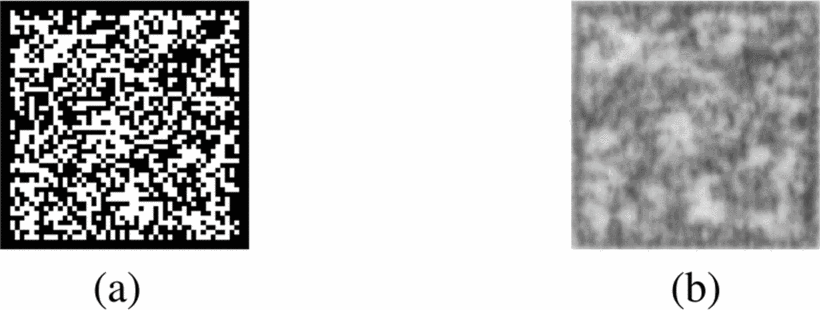
\includegraphics[width=10cm]{contents/chapter-2/2-cdporivsfake.png}
	\caption{Contoh dari CDP a) CDP original hasil \emph{generate} dari program $I$ b) CDP yang telah terdegradasi kualitasnya akibat dari beberapa kali penyetakan dan pemindaian $\widetilde{I}$ \cite{PICARDCANCOPYDETECTIONPATTERN}}
	\label{Fig: 2-cdporivsfake}
\end{figure}

\subsubsection{Prinsip Degradasi Informasi}
Prinsip dari deteksi CDP palsu dilakukan berdasarkan hilangnya informasi, yang mana muncul dari proses pemindaian dan penyetakan \cite{picard2004digital}. Proses \emph{Print-and-Scan} (P\&S) merupakan proses stokastik (mempunyai unsur peluang atau kebolehjadian) \cite{phan2014document}, yang menyebabkan perubahan struktur dan kualitas gambar pada CDP, seperti yang ditampilkan pada Gambar \ref{Fig: 2-cdporivsfake} \emph{Noise} yang dihasilkan dari P\&S CDP sulit untuk dikarakterisasi \cite{picard2008security} karena setiap printer dan pemindai memiliki karakteristiknya sendiri.

\begin{figure}[h]
	\centering
	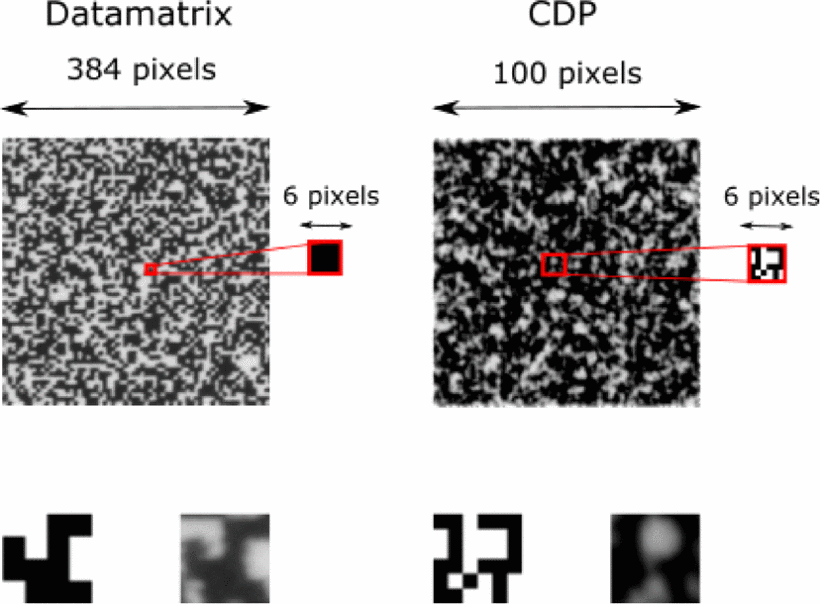
\includegraphics[width=10cm]{contents/chapter-2/2-datamatrixvscdp.png}
	\caption{Perbandingan dari CDP dengan data-matriks: Data-matriks memiliki ukuran unit komponen yang lebih besar, sehingga degradasi informasi tidak berdampak signifikan pada struktur kode \cite{PICARDCANCOPYDETECTIONPATTERN}}
	\label{Fig: 2-datamatrixvscdp}
\end{figure}

CDP sering dibandingkan dengan kode batang dua dimensi seperti data-matriks karena kemiripan visualnya. Namun, seperti yang diilustrasikan pada Gambar \ref{Fig: 2-datamatrixvscdp}, unit elemen data-matriks jauh lebih besar dibandingkan unit elemen CDP. Oleh karena itu, prinsip kehilangan atau degradasi informasi tidak berdampak pada struktur data-matriks. Sebagai contoh, korelasi antara data-matriks digital \emph{template} hasil \emph{generate} dengan versi rusak P\&S bisa lebih dari $0,9$, sedangkan korelasi antara CDP digital \emph{template} hasil \emph{generate} dengan versi rusak P\&S-nya hanya sekitar $0,45-0,55$ tergantung pada pemindai dan penyetaknya. Oleh karena itu, ukuran dari unit elemen pola CDP, yaitu $uxu$ piksel seperti yang ditampilkan pada Gambar \ref{Fig: 2-datamatrixvscdp}, ukuran pola keseluruhan juga sangat mempengaruhi proses otentikasi dan kemampuan pemalsu dalam mereproduksi pola. Pada praktiknya, ukuran unit elemen pada CDP adalah $1x1$ piksel atau $2x2$ piksel agar bisa memanfaatkan prinsip kehilangan atau degradasi informasi secara maksimal.

\subsubsection{Definisi Teoritis dari Sistem Autentikasi CDP}
Autentikasi dari CDP terdiri dari dua langkah utama. Langkah pertama adalah langkah registrasi di mana pola dihasilkan kemudian dicetak dengan penyetak untuk menghasilkan CDP asli. Langkah kedua adalah verifikasi CDP, menggunakan sebuah perangkat pemindai yang telah terotentikasi (perangkat selular dengan kamera), CDP dipindai dan dilewatkan ke tes autentikasi (dengan parameter-parameter peminadaian tertentu). Jika tes tersebut positif, item dianggap autentik.

Upaya penyerangan yang paling sering terjadi oleh pembajak adalah sebagai berikut: Pembajak melakukan pemindaian CDP pada sebuah item menggunakan pemindai beresolusi tinggi, mengestimasi pola asli dari CDP, kemudian mencetak pola yang telah diestimasi menggunakan penyetak beresolusi tinggi. Pada skenario ini $I$ merupakan CDP digital hasil \emph{generate} dari \emph{template}, kemudian $\Pi(I)$ merupakan hasil \emph{generate} CDP \emph{template} yang dicetak, dengan $\Pi(\cdot)$ \emph{noise} yang dihasilkan dalam proses penyetakan menggunakan penyetak yang telah terautentikasi. Selanjutnya, proses autentikasi dapat dirumuskan sebagai uji hipotesis berikut ini:

\begin{align}
	&\mathcal{H}_{0}:\tilde{I}\sim\Sigma(\Pi(I)),\\ &\mathcal{H}_{1}:\tilde{I}\not\sim\Sigma(\Pi(I)),\nonumber
\end{align}

\noindent di mana $\widetilde{I}$ adalah gambar CDP \emph{grayscale} yang diterima oleh pusat autentikasi. $\widetilde{I}$ dapat berupa CDP asli (i.e. $\Sigma(\Pi(I))$) atau CDP palsu (i.e. $\Sigma(\Pi'(\hat{I}))$). Metriks yang digunakan untuk membandingkan CDP asli dengan palsu adalah koefisien jarak ataupun korelasi \cite{dirik2012copy}.

\subsubsection{Komponen dari Detektor}
Hasil menunjukkan bahwa autentikasi menggunakan CDP \emph{raw grayscale} lebih efisien dibandingkan dengan CDP yang telah di-\emph{thresholding} \cite{phan2014document}. Kemudian, secara umum, ada beberapa langkah yang dilakukan untuk melakukan autentikasi CDP, antara lain:

\begin{itemize}
	\item Melakukan \emph{resizing} pada \emph{template} CDP menggunakan faktor skala tertentu.
	\item Menggunakan teknik pencocokan \emph{template} dengan mengambil sub-bagian dari CDP.
	\item Menggunakan \emph{high pass filtering} (seperti \emph{unsharp masking}) sebelum melakukan penyekoran korelasi.
\end{itemize}

\subsection{Detekti Pembajakan menggunakan SQR}
Pendekatan keamanan tradisional pada produk sebelumnya sudah diimplementasikan melalui \emph{taggant}, hologram, dan tinta keamanan.Beberapa metode tersebut memang mudah diimplementasikan, mudah diverifikasi, dan murah. Namun, dalam sebuah Kode QR metode-metode tersebut belum dapat diimplementasikan. Produk yang ditempeli oleh kode QR palsu biasanya masih dapat dipindai dan mengembalikan keluaran sama dengan produk asli. Penelitian yang dilakukan oleh Justin Picard, Paul Landry, dan Michael Bolay ini membahas tentang bagaimana mengimplementasikan CDP ke dalam SQR untuk mendeteksi pembajakan \cite{picard2021counterfeit}.

\begin{figure}[h]
	\centering
	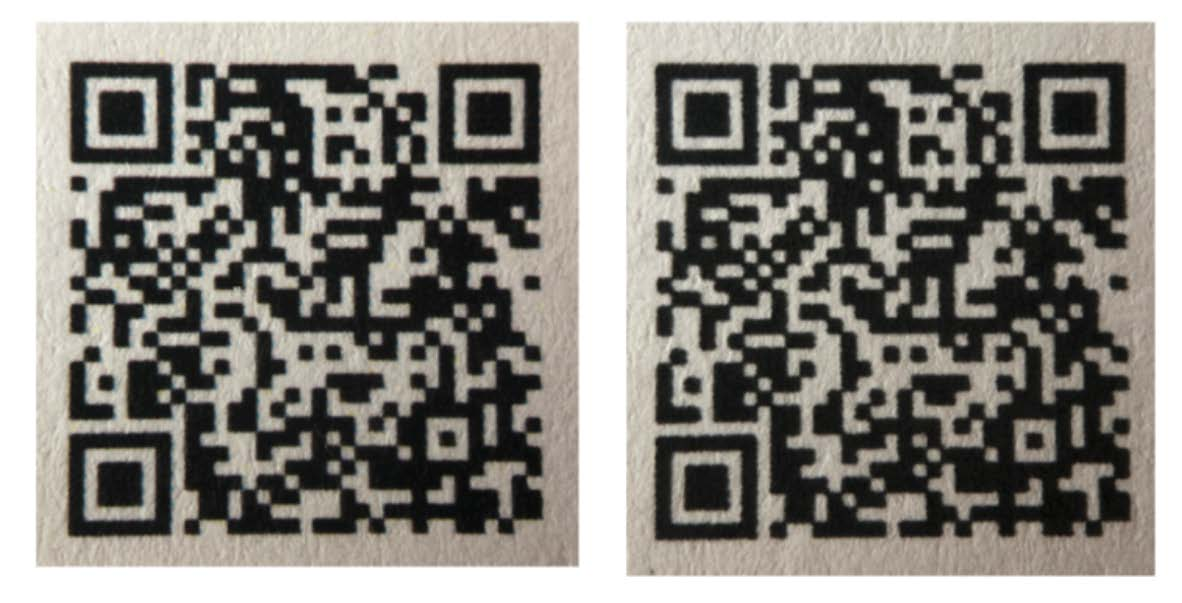
\includegraphics[width=10cm]{contents/chapter-2/2-qrorivspalsu.jpg}
	\caption{Perbandingan dari kode QR asli dan palsu, keduanya menyimpan informasi yang sama dan sama-sama dapat dipindai \cite{picard2021counterfeit}}
	\label{Fig: 2-qrorivspalsu}
\end{figure}

Pada Gambar \ref{Fig: 2-qrorivspalsu} terlihat bahwa sangat sulit untuk membedakan antara kode QR asli dan replika, apabila jika tidak ada pembandingnya. Skenario yang dapat dilakukan oleh pembajak dalam menerbitkan kode QR palsu dapat dilihat pada Gambar \ref{Fig: 2-counterveiterpractice}. Kode QR palsu dipindai dengan perangkat beresolusi tinggi, kemudian dicetak ulang. Harapannya dengan CDP yang diletakkan pada kode QR, kode QR palsu yang dipindai untuk autentikasi dapat terdeteksi sebagai kode QR palsu, lihat pada Gambar \ref{Fig: 2-counterveiterpractice}.

\begin{figure}[h]
	\centering
	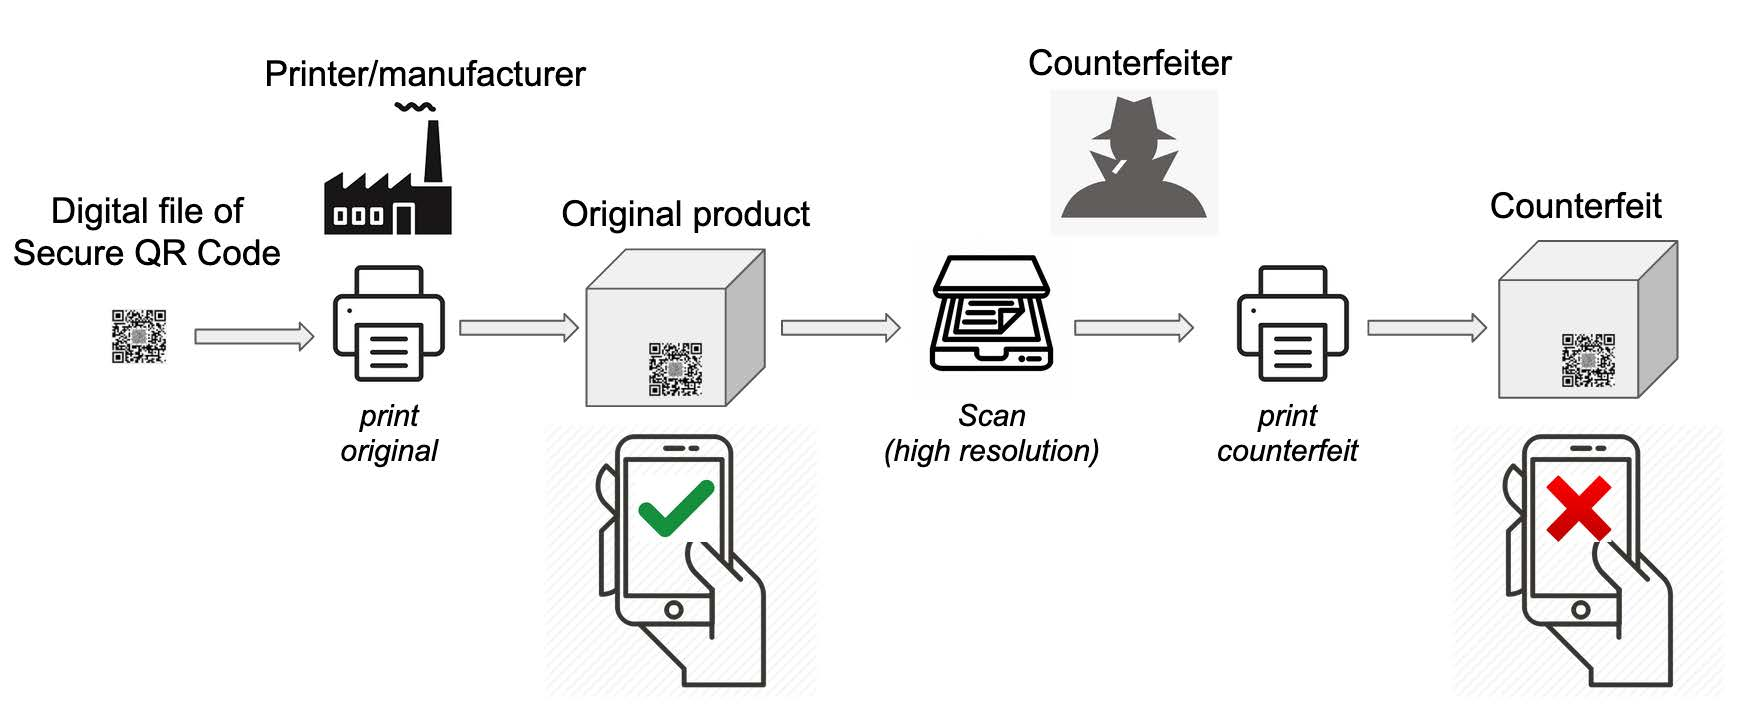
\includegraphics[width=10cm]{contents/chapter-2/2-counterveiterpractice.jpg}
	\caption{SQR diharapkan dapat mendeteksi kode QR palsu pada saat diautentikasi oleh pengguna \cite{picard2021counterfeit}}
	\label{Fig: 2-counterveiterpractice}
\end{figure}

\subsubsection{Struktur dari SQR}
\begin{figure}[h]
	\centering
	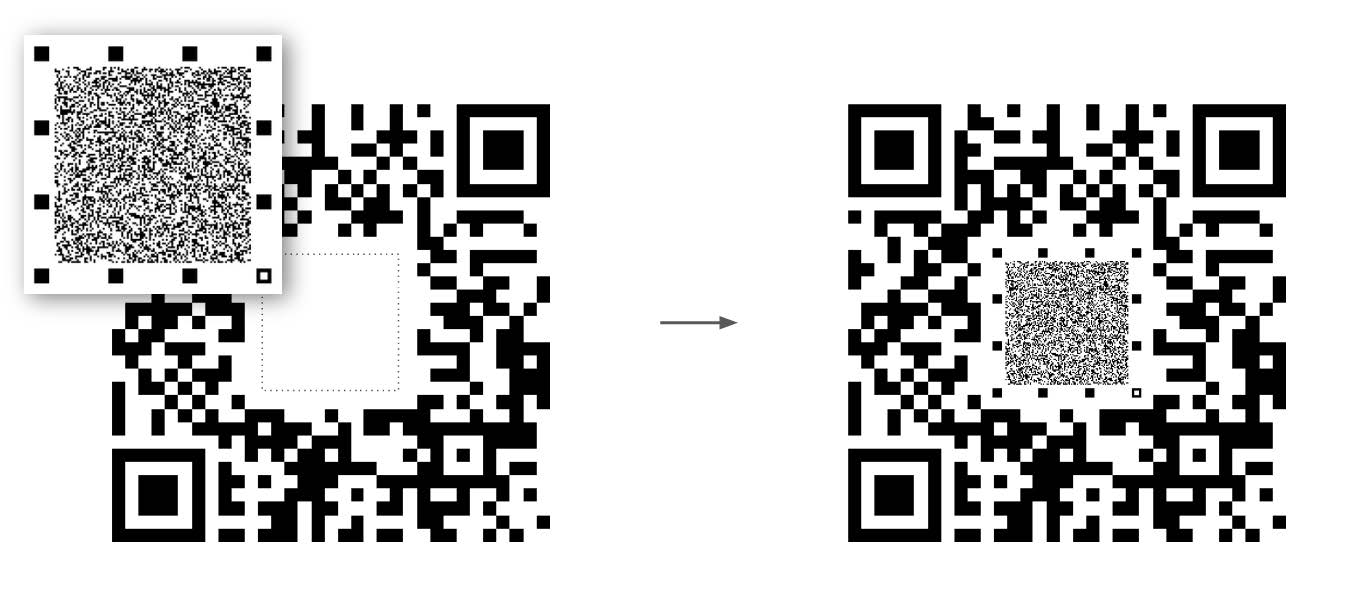
\includegraphics[width=10cm]{contents/chapter-2/2-struktursqr.jpg}
	\caption{Struktur SQR secara umum \cite{picard2021counterfeit}}
	\label{Fig: 2-struktursqr}
\end{figure}

Secara umum, CDP akan diletakkan di tengah-tengah dari kode QR. CDP nantinya akan digunakan untuk proses autentikasi. Di sekitar CDP diletakkan beberapa \emph{markers} untuk memudahkan program dalam mendeteksi dan mendapatkan objek CDP. CDP mungkin ditempelkan di tengah-tengah kode QR karena adanya fitur koreksi kesalahan dalam kode QR. Ada empat jenis koreksi kesalahan pada kode QR: L, M, Q, dan H, yang secara teoritis memiliki kemampuan untuk memulihkan informasi yang hilang sebesar 7\%, 15\%, 25\%, dan 30\% kerusakan pada kode QR. Pada penelitian ini, area yang dirusak untuk meletakkan CDP adalah sebesar 1/9 dari ukuran awal kode QR. Aplikasi yang digunakan untuk melakukan autentikasi pada perangkat pemindai (perangkat seluluer) hanya mengambil objek CDP saja, hal tersebut memiliki beberapa keuntungan, area yang digunakan untuk autentikasi menjadi lebih spesifik, sehingga kecepatan deteksi akan lebih cepat, fokus dari kamera juga relatif akan lebih baik karena mengambil objek yang lebih kecil dan terfokus, selain itu karena sistem autentikasi berada di \emph{remote server} yang mana data akan dikirim dari perangkat seluler pemindai, maka semakin kecil area yang dikirimkan, semakin hemat \emph{bandwith} yang digunakan.

\subsubsection{Pembuatan dan Pencetakan SQR}
CDP yang digunakan dalam penelitian ini menggunakan dua kuantisasi \emph{grayscale} atau biner. Resolusi mesin \emph{printer} yang digunakan adalah 812,8 ppi dengan merek HP Indigo. CDP di-\emph{generate} menggunakan \emph{pseudo-random number generator}, menggunakan \emph{seed} tertentu. CDP dapat dibuat unik untuk setiap kode QR ataupun sama pada sekelompok kode QR tertentu. Dalam melakukan penyetakan dan pemindaian SQR, perangkat pencetak dan pemindai akan diverifikasi terlebih dahulu dengan konfigurasi dan parameter tertentu untuk menjamin kualitas dari pencetakan.

\subsubsection{Autentikasi SQR}
Perangkat pemindai QR biasa sudah pasti dapat melakukan \emph{decode} informasi dari kode QR, namun untuk melakukan autentikasi terhadap CDP, tentunya diperlukan aplikasi khusus. Aplikasi khusus ini berjalan di perangkat seluler, secara umum proses pemindaian yang dilakukan oleh aplikasi khusus tersebut adalah sebagai berikut:

\begin{itemize}
	\item Aplikasi akan melakukan pemindaian per-\emph{frame} dari kamera hingga mendapatkan kode QR.
	\item Kode QR akan di-\emph{decode} untuk mengekstrak informasi dalam kode QR.
	\item Indeks kualitas pemindaian akan dikalkulasi berdasarkan \emph{frame} yang didapatkan.
	\item Jika indeks kualitas pemindaian dinilai cukup tinggi, area CDP akan dideteksi, dipotong, dan dikirim ke \emph{remote server} bersamaan dari informasi dari kode QR yang telah ter-\emph{decode} untuk autentikasi.
\end{itemize}

\begin{figure}[h]
	\centering
	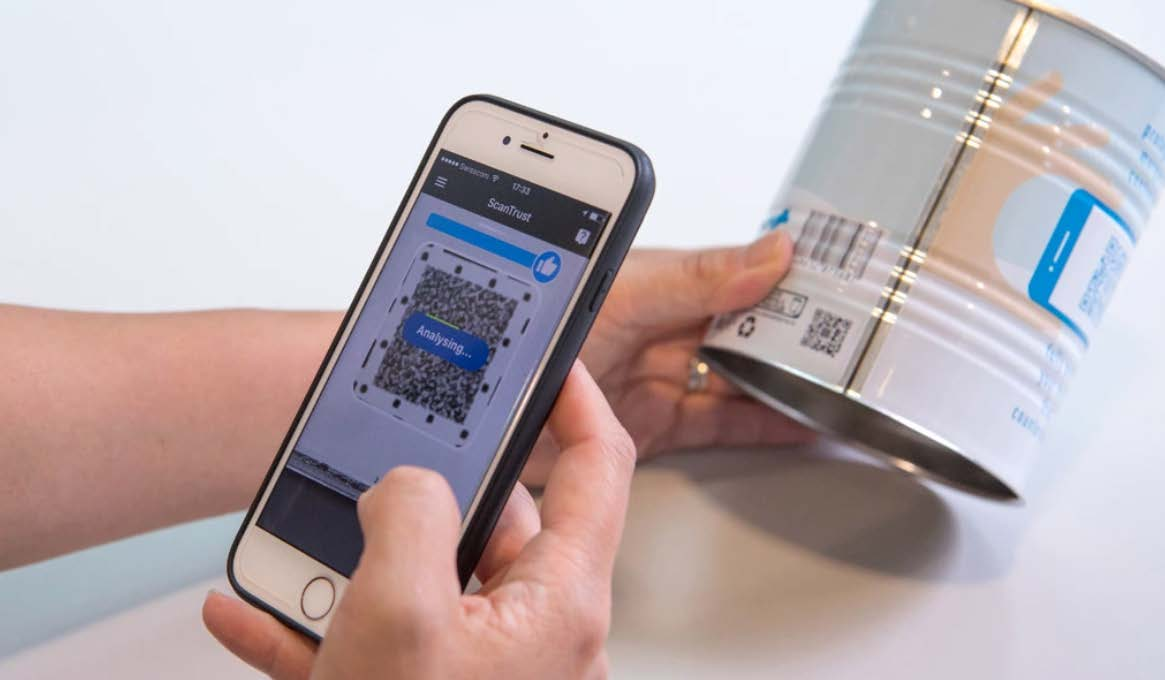
\includegraphics[width=10cm]{contents/chapter-2/2-pemindaiansqr.jpg}
	\caption{Perangkat seluler melakukan pemindaian menggunakan aplikasi khusus \cite{picard2021counterfeit}}
	\label{Fig: 2-pemindaisqr}
\end{figure}

Setelah \emph{server} mendapatkan CDP yang telah dipotong beserta informasi data kode QR, autentikasi yang dilakukan di \emph{server} adalah sebagai berikut:

\begin{itemize}
	\item \emph{Identifier} unik akan diekstrak dari informasi kode QR yang didapatkan yang mana dibutuhkan sebagai parameter autentikasi.
	\item Template CDP digital akan di-\emph{generate}.
	\item Matriks similaritas akan dikalkulasi dari perbandingan antara CDP yang dikirimkan dari hasil pemindaian dengan CDP \emph{template} yang di-\emph{generate}.
	\item Penyesuaian lain seperti, ketajaman gambar, filter akan dilakukan untuk memperoleh hasil terbaik.
	\item Normalisasi nilai akan dilakukan.
	\item Keluaran berupa CDP "asli", "palsu", atau "pemindaian buruk" akan dikeluarkan oleh \emph{server} (pemindaian buruk bisa disebabkan oleh hasil gambar yang blur).
\end{itemize}

\subsection{Autentikasi Digital menggunakan CDP}

\subsection{Pencetakan Variasi CDP}

\subsection{Autentikasi CDP menggunakan Perangkat Seluler}

\section{Dasar Teori}

\subsection{Kode QR}

Kode QR (Quick Response) adalah sebuah kode matriks dua dimensi (2-D) yang dapat dibaca oleh komputer. Kode QR dua dimensi dapat menyimpan data yang lebih banyak dibandingkan dengan kode satu dimensi (barcodes) dengan ruang yang lebih kecil. Selain itu, kode QR memiliki fitur koreksi kesalahan pembacaan dan beberapa fitur unik lainnya \cite{densoqrcode}. 

Seperti bahasa tertulis lainnya, kode batang atau \emph{barcode} merupakan representasi visual dari informasi. Namun, berbeda dengan bahasa yang dapat dibaca oleh manusia, kode batang dirancang untuk dibaca dan dipahami oleh komputer atau mesin. Menggunakan sistem penglihatan dari mesin berupa pemindai laser optik ataupun kamera dan perangkat lunak yang dapat menginterpretasikan kode batang. Aturan bagaimana \emph{barcode} dikonstruksikan disebut sebagai \emph{grammar}, sedangkan set karakter yang digunakan (alfabet) disebut \emph{symbology} \cite{densoqrcode}.

\subsubsection{Bagaiamana Kode QR Bekerja}
\begin{figure}[h]
	\centering
	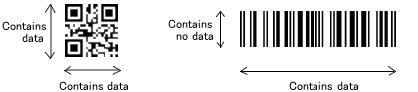
\includegraphics[width=10cm]{contents/chapter-2/2-2dvs1dcode.jpg}
	\caption{Perbandingan 1-D dengan 2-D \emph{barcodes}}
	\label{Fig: 2-2dvs1dcode}
\end{figure}

Tidak seperti kode batang satu dimensi, kode QR adalah matriks 2-D yang menyimpan informasi dalam tiap modul di baris dan kolomnya yang memiliki gelap dan terang tertentu.

\begin{figure}[h]
	\centering
	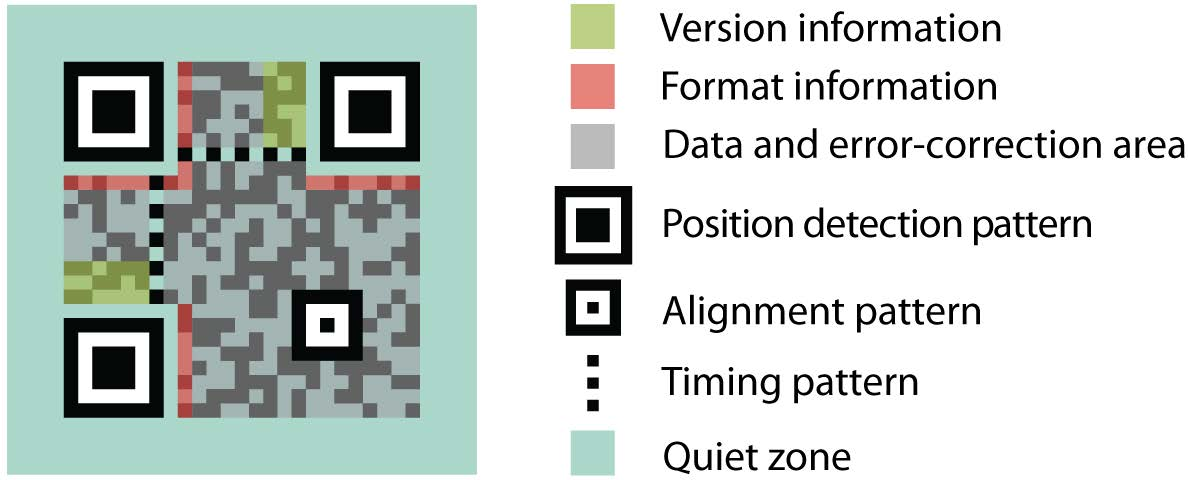
\includegraphics[width=10cm]{contents/chapter-2/2-strukturqrasli.jpg}
	\caption{Struktur modul pada kode QR dua dimensi}
	\label{Fig: 2-strukturqrasli}
\end{figure}

Setiap modul dalam kode QR memiliki fungsi-fungsi tertentu. Beberapa modul berisi tentang informasi yang tersimpan dalam kode QR itu sendiri, dengan lainnya dibagi menjadi beberapa grup berdasarkan fungsinya. Untuk memastikan kode QR dapat dipindai dari berbagai sisi, ada tiga modul \emph{position detection pattern} yang terletak di ketiga sudut yang memungkinkan kode QR untuk dipindai dari 360$^{\circ}$.

\subsubsection{Versi Kode QR}
Kode QR dapat di-\emph{generate} dari 40 versi yang berbeda, dari yang berukuran $21x21$ modul (versi 1) hingga $177x177$ modul (versi 40).

\begin{figure}[h]
	\centering
	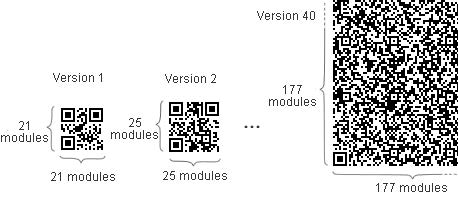
\includegraphics[width=10cm]{contents/chapter-2/2-versiqr.jpg}
	\caption{Jumlah modul berdasarkan versi kode QR}
	\label{Fig: 2-versiqr}
\end{figure}

Setiap kenaikan satu versi, maka akan ada penambahan 4 modul, sehingga dapat memuat data atau informasi yang lebih banyak. Jumlah maksimum data yang dapat disimpan tergantung pada versi kode QR, tipe karakter, dan besar toleransi kesalahan.

\subsubsection{Koreksi Kesalahan Kode QR}
Koreksi kesalahan kode QR mengimplementasikan \emph{Reed-Solomon codes}, yang mana merupakan salah satu metode koreksi kesalahan matematis yang banyak digunakan. Hal ini memungkinkan kode QR tetap dapat dibaca walaupun dalam kondisi kotor ataupun rusak dengan batasan tertentu. Ada empat tipe koreksi kesalahan standar yang ada dalam kode QR. Semakin tinggi level koreksi kesalahan, semakin besar toleransi terhadap kerusakan kode QR, namun semakin besar juga versi kode QR-nya.

\begin{table}[h]
	\caption{Tabel perbandingan level koreksi kesalahan dengan persentase toleransi kesalahannya}
	\vspace{0.5em}
	\centering
	\begin{tabular}{|c|c|c|}
		\hline
		Level Koreksi Kesalahan & Besar Toleransi Kesalahan \\
		\hline
		L & 7\% \\
		M & 15\% \\
		Q & 25\% \\
		H & 30\% \\ \hline
	\end{tabular}
	\label{Tab: 2-tabelperbandinganlevelkoreksi}
\end{table}

Dalam memilih level koreksi kesalahan, sebaiknya disesuaikan dengan kondisi lingkungan di mana kode QR tersebut digunakan. Misalnya dalam kondisi lingkungan yang bersih, level L (7\%) dapat digunakan. Secara umum, level yang paling sering digunakan adalah level M (15\%).

\subsection{Deteksi Pola Duplikat (CDP)}
Pola deteksi duplikat (CDP) adalah sebuah gambar berpola dengan entropi tinggi yang dibuat menggunakan kode rahasia (\emph{secret key}). CDP memanfaatkan konsep dari "\emph{information loss principle}" dari proses P\&S pada dokumen. Biasanya, CDP digunakan di dalam gambar digital yang dicetak ataupun langsung ke dalam dokumen digitalnya. CDP tidak didesain untuk dideteksi menggunakan mata telanjang. Namun, CDP dapat bekerja secara maksimal pada pendeteksian otomatis pada gambar yang dipindai. CDP akan sangat bermanfaat saat digunakan dalam memverifikasi dokumen dalam jumlah besar \cite{picard2004digital}, \cite{picard2004towards}, \cite{}.

\begin{figure}[h]
	\centering
	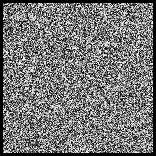
\includegraphics[width=3cm]{contents/chapter-2/2-contohcdp.jpg}
	\caption{Salah satu contoh CDP}
	\label{Fig: 2-contohcdp}
\end{figure}

CDP telah dicoba untuk dicetak menggunakan berbagai variasi \emph{printers}: \emph{Printer} kantor seperti \emph{inkjet} dan \emph{laser}, \emph{printer offset} dan \emph{digital offset}, dan juga \emph{printer} termal. Hasil percobaan dari pencetakan menggunakan beberapa jenis \emph{printer} tadi, semua CDP salinan dapat dibedakan dengan CDP asli dengan margin yang cukup nyaman \cite{picard2004digital}, \cite{picard2004towards}.

CDP sebaiknya tidak dianggap sebagai pesaing untuk perangkat keamanan optik lainnya, namun dijadikan sebagai alternatif yang lebih murah pada kasus-kasus tertentu. Dengan memanfaatkan konsep degradasi gambar dan informasi yang tidak terancam oleh perkembangan perangkat pemindai dan pencetak digital, CDP menjadi alternatif yang paling murah dalam memroteksi dokumen \cite{picard2004digital}, \cite{picard2004towards}, \cite{harwood1998optical}.

\subsection{Lokalisasi Objek dengan Pengenalan Pola}
Lokalisasi objek adalah proses mengidentifikasi posisi dan orientasi objek atau pola tertentu pada sebuah gambar menggunakan teknik pengolahan citra dan visi komputer. Proses ini melibatkan deteksi objek atau pola dalam gambar serta mengestimasi lokasi dan orientasi yang tepat relatif terhadap kamera \cite{sivic2003video}, \cite{liu2016ssd}.

Berbagai teknik telah diusulkan untuk melakukan lokalisasi objek atau gambar dengan pengenalan pola, termasuk deteksi fitur, pencocokan \emph{template}, dan metode berbasis pembelajaran mesin. Teknik-teknik ini telah digunakan dalam berbagai aplikasi, seperti \emph{augmented reality}, robotika, dan pelacakan objek.

\subsection{ArUco \emph{Marker}}
ArUco \emph{marker} adalah jenis \emph{marker} fidusial yang biasa digunakan untuk estimasi pose kamera dan pelacakan dalam pengolahan citra dan visi komputer. ArUco \emph{marker} terdiri dari kisi-kisi kotak hitam dan putih dengan pola unik yang mudah dideteksi dan dikenali oleh algoritma visi komputer. ArUco \emph{marker} banyak digunakan dalam aplikasi robotika, realitas tambahan, dan pelacakan objek karena kesimpelannya, akurasi deteksi yang tinggi, dan biaya komputasi yang rendah.

\emph{Marker} fidusial adalah objek berpola yang digunakan ke dalam sebuah gambar atau tempat tertentu untuk memudahkan sistem visi komputer menentukan posisi dan orientasi objek atau \emph{scene} dengan akurasi yang tinggi. \emph{Marker} fidusial biasanya didesain dengan pola atau bentuk yang unik dan mudah dikenali, sehingga dapat dideteksi dan dilacak oleh algoritme pendeteksian objek visi komputer, yang memungkinkan estimase pose dan pelacakan yang akurat. \emph{Marker} fidusial banyak digunakan dalam berbagai aplikasi seperti \emph{augmented reality}, robotika, dan pendeteksian objek.

% \subsection{Ekstraksi Fitur pada Gambar}

\subsection{Koefisien Jarak}
Koefisien jarak merupakan ukuran atau besaran yang menggambarkan seberapa dekat atau jauh dua objek dalam ruang atau dimensi tertentu. Koefisien jarak dapat digunakan untuk mengukur kesamaan atau perbedaan antara dua objek yang diamati. Ada beberapa koefisien jarak yang sering digunakan, antara lain:

\subsubsection{Koefisien Jarak Euclidean}
Jarak Euclidean adalah ukuran jarak yang paling umum digunakan dalam matematika dan ilmu komputer untuk mengukur jarak antara dua titik dalam ruang Euclidean n-dimensi. Jarak Euclidean dihitung sebagai akar kuadrat dari jumlah kuadrat perbedaan koordinat antara dua titik.
Secara formal, jarak Euclidean antara dua vektor $\mathbf{u}$ dan $\mathbf{v}$ dalam ruang Euclidean n-dimensi didefinisikan sebagai:

\begin{equation}
  d(\mathbf{u},\mathbf{v}) = \sqrt{\sum_{i=1}^{n}(u_i - v_i)^2}
\end{equation}

\noindent di mana $n$ adalah jumlah dimensi dalam \emph{vector space}, dan $u_i$ dan $v_i$ merepresentasikan komponen ke-$i$ pada vektor.

\subsubsection{Koefisien Jarak Korelasi}
Koefisien jarak korelasi adalah suatu ukuran kemiripan atau perbedaan antara dua vektor, berdasarkan korelasi antara komponen-komponennya. Nilai dari jarak korelasi dinormalisasi antara 0 dan 1, di mana 0 menunjukkan korelasi positif sempurna sedangkan 1 menunjukkan korelasi negatif sempurna.

Untuk menghitung jarak korelasi antara dua vektor $u$ dan $v$, dapat dituliskan dengan:

\begin{equation}
	d = 1-\frac{(u-\bar{u})\cdot (v-\bar{v})}{\Vert(u-\bar{u})\Vert_2\Vert(v-\bar{v})\Vert_2}
\end{equation}

\noindent di mana $d$ adalah jarak korelasi antara $u$ dan $v$, $\bar{v}$ adalah rata-rata elemen dari vektor $v$, dan $x\cdot y$ adalah \emph{dot product} dari $x$ dan $y$. Jarak korelasi sering digunakan dalam algoritma pengelompokan dan klasifikasi untuk mengukur perbedaan antara sampel, terutama ketika vektor memiliki banyak komponen dan data sangat berkorelasi.

\subsubsection{Koefisien Jarak Kosinus}
Koefisien jarak kosinus adalah sebuah metode untuk mengukur kemiripan antara dua vektor dalam ruang n-dimensi \cite{schutze2008introduction}, \cite{deisenroth2020mathematics}. Metode ini mengukur sudut antara dua vektor dan menghasilkan nilai berkisar antara 0 dan 1, di mana 0 menunjukkan bahwa vektor tersebut saling tegak lurus, sedangkan 1 menunjukkan bahwa vektoor tersebut saling sejajar. Semakin kecil nilai koefisien jarak kosinus, semakin mirip kedua vektor tersebut. Jarak kosinus antara dua vektor $u$ dan $v$ dapat dituliskan sebagai berikut:

\begin{equation}
	1-\frac{u\cdot v}{\Vert u\Vert_2\Vert v\Vert_2}
\end{equation}

\noindent di mana $u\cdot v$ adalah hasil \emph{dot product} antara vektor $u$ dan $v$, sedangkan $\Vert u\Vert_2$ dan $\Vert v\Vert_2$ adalah panjang dari vektor $u$ dan $v$.

\subsubsection{Koefisien Jarak Canberra}
Jarak Canberra adalah salah satu metode mengukur jarak antara dua vektor dalam ruang n-dimensi. Metode ini mengevaluasi perbedaan proporsional antara nilai-nilai pada setiap elemen vektor. Metode ini sering digunakan dalam analisis data untuk mengukur kemiripan antara dua set data numerik \cite{clusteringSumayiaAlAnazi}, \cite{sneath1973numerical}. Secara formal, perhitungan jarak canberra antara dua vektor $u$ dan $v$ adalah:

\begin{equation}
	d(u,v)=\sum_i\frac{\left | u_i-v_i \right |}{\left | u_i \right |+\left | v_i \right |}
\end{equation}

\subsection{Transformasi Homografi}
Transformasi homografi adalah sebuah transformasi geometri pada ruang n-dimensi yang memetakan setiap titik pada bidang ke titik yang sesuai pada bidang lainnya, dengan menerapkan konsep persamaan linier homogen. Transformasi homografi dapat mengubah ukuran, rotasi, dan persepektif dari gambar atau objek pada bidang ruang n-dimensi.

Transformasi homografi biasanya dilakukan dalam ruang koordinat \emph{homogeneous}, yang merupakan ruang n+1 dimensi dengan koordinat homogen yang memungkinkan dilakukannya transformasi perspektif. Dalam ruang koordinat \emph{homogeneous}, sebuah titik pada bidang n-dimensi dinyatakan dalam bentuk vektor homogen (x, y, z, w), di mana x, y, dan z adalah koordinat euclidean, dan w adalah koordinat homogen. Sebuah matriks homografi H juga dinyatakan dalam bentuk matriks homogen:

\begin{equation}
	\begin{bmatrix}
		x'\\ 
		y'\\ 
		w'
		\end{bmatrix}=H\begin{bmatrix} 
		x\\ 
		y\\ 
		w
		\end{bmatrix}
\end{equation}

\subsection{Pembelajaran Mesin}


\section{Analisis Perbandingan Metode}
\chapter{Metode Penelitian}
Secara umum, tujuan dari penelitian ini adalah menguji performa dari CDP dengan dua dan empat kuantisasi \emph{grayscale}. Selain itu, penelitian ini juga menguji performa penggunaan enam ArUco \emph{marker} di sekitar CDP dalam membantu proses lokalisasi objek CDP. Dalam prosesnya, metode-metode penelitian yang dirancang dan dilakukan penulis akan dijelaskan pada bab ini.

\section{Alat dan Bahan Tugas Akhir}

\subsection{Alat Tugas Akhir}

Alat yang digunakan pada penelitian ini terbagi atas perangkat keras dan perangkat lunak yang dengan rincian sebagai berikut:

\begin{enumerate}
	\item Laptop Lenovo Legion Y530\\Merupakan perangkat keras utama yang digunakan dalam penelitian. Laptop ini memiliki spesifikasi sebagai berikut: Prosesor Intel I5-8300H, RAM 8 GB DDR4, Kartu Grafis Nvidia Geforce GTX 1050TI (4 GB).
	\item Python 3.9\\Perangkat lunak yang merupakan bahasa pemrograman utama yang digunakan dalam mengembangkan model SQR dan membuat model untuk melakukan klasifikasi SQR asli dan palsu.
	\item Microsoft Visual Studio Code\\Merupakan salah satu perangkat lunak editor kode sumber terpopuler dan gratis yang dikembangkan oleh Microsoft. Editor ini memiliki berbagai fitur yang memungkinkan pengguna untuk menulis, mengedit, dan mengelola kode sumber dengan mudah dan efisien. Selain itu, editor ini juga mendukung berbagai bahasa pemrograman, termasuk JavaScript, Python, Java, C++, dan masih banyak lagi. Tampilan antarmuka pengguna VS Code sangat bersih dan dapat disesuaikan, sehingga pengguna dapat mengatur tata letak dan tema yang sesuai dengan preferensi mereka. Selain itu, editor ini juga mendukung berbagai bahasa pemrograman, termasuk JavaScript, Python, Java, C++, dan masih banyak lagi. Fitur-fitur kunci dari VS Code termasuk kemampuan untuk mengeksekusi kode secara langsung dari editor, penyelesaian otomatis kode, refaktoring kode, debugging, pengelolaan paket, dan integrasi dengan sistem kontrol versi seperti Git.
	\item Jupyter Notebook \emph{Ekstension} \emph{for} VS Code\\Merupakan perangkat lunak ekstensi untuk visual studio code untuk menjalankan jupyter notebook di dalam \emph{environment} visual studio code.
	\item Adobe Acrobat DC\\Merupakan perangkat lunak yang digunakan sebagai pembaca dan pengedit fail PDF. Perangkat lunak ini banyak penulis gunakan untuk mengubah ukuran \emph{batch} QR menjadi ukuran standar percetakan.
	\item Adobe Photoshop 2022\\Merupakan perangkat lunak yang digunakan sebagai editor gambar. Perangkat lunak ini penulis gunakan dalam penelitian untuk mengubah fail PNG hasil \emph{generate batch} QR dari kode menjadi PDF. 
	\item \emph{Smartphone} Realme GT Neo 3T\\Perangkat keras yang digunakan sebagai pemindai SQR dalam pembuatan \emph{dataset} SQR asli dan palsu. \emph{Smartphone} ini memiliki spesifikasi sebagai berikut: \emph{Chipset} Qualcomm SM8250-AC Snapdragon 870 5G, sistem operasi Android 12, kamera utama dengan resolusi 64 MP, f/1.8, 25mm.
	\item \emph{Printer} Xerox Versant\\Perangkat keras yang digunakan sebagai pencetak utama \emph{dataset} SQR asli dan palsu. \emph{Printer} ini merupakan \emph{printer} berspesifikasi tinggi yang banyak digunakan dalam industri percetakn.
	\item Boks\\Boks digunakan sebagai \emph{environment} yang digunakan untuk menstandarisasi hasil pemotretan atau pemindaian \emph{dataset} SQR menggunakan kamera \emph{smartphone}.
	\item Gunting\\Gunting digunakan untuk memotong \emph{dataset} SQR yang nantinya akan dipotret.
\end{enumerate}

\subsection{Bahan Tugas akhir}
\begin{enumerate}
	\item \emph{Dataset} SQR dengan Dua Level \emph{Grayscale}
	\item \emph{Dataset} SQR dengan Empat Level \emph{Grayscale}
\end{enumerate}

Bahan yang digunakan pada penelitian ini terbagi atas perangkat keras dan perangkat lunak yang dengan rincian sebagai berikut:

\section{Metode yang Digunakan}

\subsection{Pembuatan Model SQR Orisinal}
Model SQR yang coba dikembangkan oleh penulis adalah menempelkan \emph{watermark} di tengah-tengah kode QR biasa. \emph{Watermark} yang ditempelkan merupakan gabungan dari CDP dan juga enam ArUco \emph{markers} untuk membantu lokalisasi objek CDP. CDP yang ditempelkan pada kode QR digunakan untuk autentikasi, apakah SQR tersebut orisinal ataukah palsu. Secara umum, desain dari SQR yang dirancang oleh penulis dapat dilihat pada

\subsubsection{Penentuan Versi Kode QR}
Setiap versi dari kode QR memiliki kapasitas penyimpanan data yang berbeda, kode QR versi 1 memiliki ukuran $21x21$ modul, sedangkan kode QR versi 40 memiliki ukuran $177x177$ modul. Setiap kenaikan satu versi kode QR, maka akan ada penambahan sebanyak 4 modul, misalkan kode QR versi 1 memiliki jumlah modul $21x21$, maka kode QR versi 2 memiliki jumlah modul $25x25$, kode QR versi 3 memiliki jumlah modul $29x29$, dan seterusnya. Semakin banyak modul yang dimiliki kode QR, semakin banyak juga data yang dapat disimpan.

\subsubsection{Penentuan Level PCT}
PCT level merupakan ukuran untuk seberapa banyak kode QR akan dirusak untuk ditempeli \emph{watermark}. Karena \emph{watermark} yang didesain berukuran $172x172$ piksel, sedangkan ukuran kode QR dengan \emph{box\_size} 20 dan jumlah modul 29 sesuai dengan jumlah modul kode QR versi 3. Karena \emph{watermark} yang didesain berukuran $172x172$, maka level koreksi kesalahan yang digunakan adalah level H atau sama dengan 30\% koreksi kesalahan yang ditolerir. Jumlah modul yang dapat dirusak atau ditolerir kerusakannya oleh koreksi kesalahan level H adalah:

\begin{align}
	n &= n_v.b_s\\&=29.20\nonumber\\&=580\nonumber\\di mana:\\n &= Jumlah akhir modul kode QR\\n_v &= Jumlah modul pada versi kode QR v\\b_s &= Ukuran \emph{box size}
\end{align}
di mana:



\begin{conditions*}
	n & Ukuran piksel kode QR\\
	n & Ukuran piksel kode QR
\end{conditions*}

\subsubsection{Penentuan Ukuran SQR yang Dirusak}

\subsubsection{Pembuatan CDP}

\subsubsection{Pembuatan ArUco \emph{Marker} di Sekitar CDP}

\subsubsection{Peletakan \emph{Watetermark} di Kode QR}

\subsection{Pembuatan}

\subsection{Pengujian Ukuran ArUco \emph{Marker}}

\section{Alur Tugas Akhir}

Menguraikan prosedur yang akan digunakan dan jadwal atau alur penyelesaian setiap 
tahap. Alur penelian ini dapat disajikan dalam bentuk diagram. Diagram dapat disusun dengan aturan yang baik semisal menggunakan \textit{flowchart}. Aturan dan tutorial pembuatan \textit{flowchart} dapat dilihat di \textcolor{blue}{http://ugm.id/flowcharttutorial}. Setelah menggambarkannya, penulis wajib menjelaskan langkah-langkah setiap alur tugas akhir dalam sub bab tersendiri sesuai dengan kebutuhan.

\chapter{Hasil dan Pembahasan}

\section{Hasil Akhir Desain SQR}

\begin{figure}[h]
	\centering
	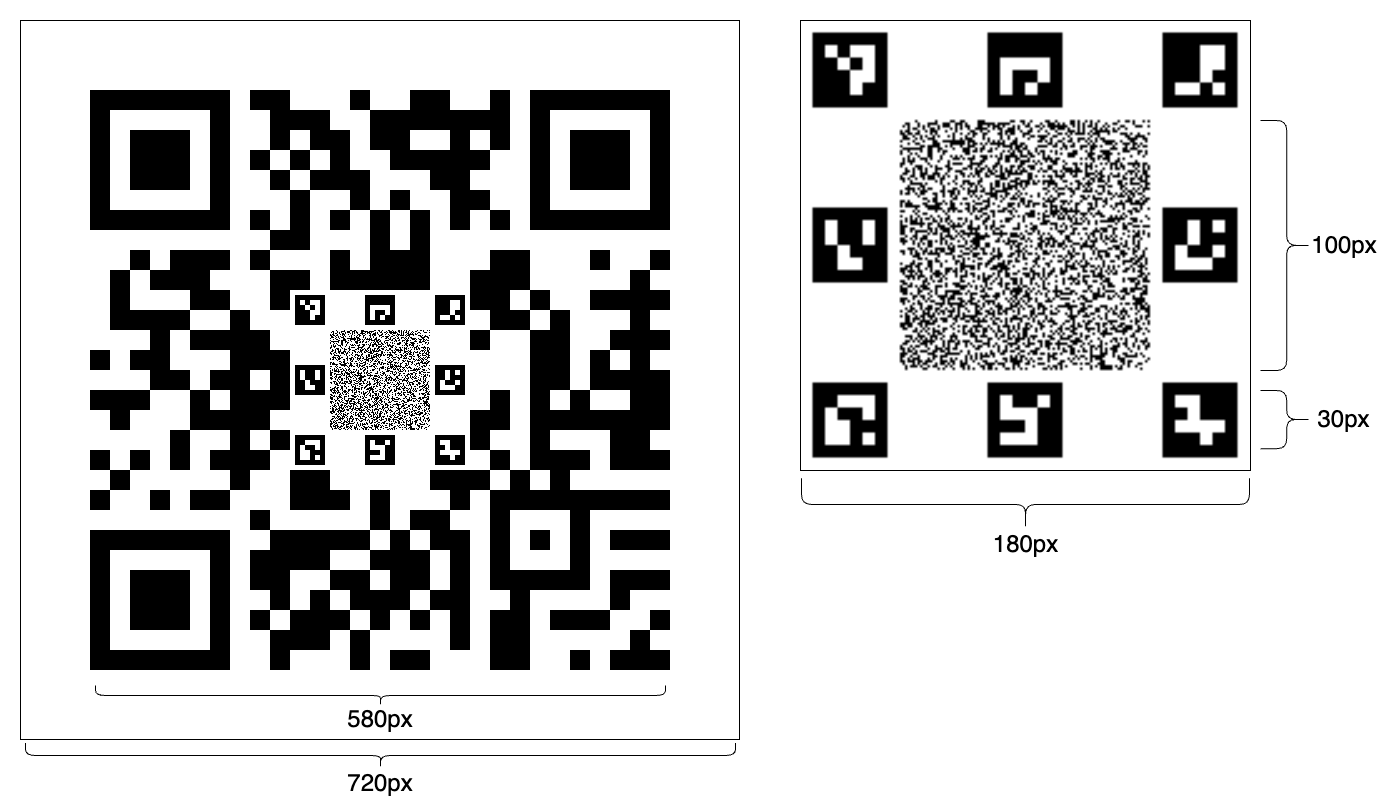
\includegraphics[width=12cm]{contents/chapter-4/4-modelsqrfinal.png}
	\caption{Hasil akhir desain SQR}
	\label{Fig: 4-modelsqrfinal}
\end{figure}

Hasil akhir dari desain SQR yang penulis buat dapat dilihat pada Gambar \ref{Fig: 4-modelsqrfinal}. Versi kode QR yang digunakan adalah kode QR versi 3, dengan
29 modul dan 20 \emph{box-size}, sehingga jika dikalikan ukurannya menjadi 580 x 580 piksel. Selain itu, ditambahkan \emph{padding} berukuran 70 piksel,
sehingga ukuran total dari SQR adalah 720 x 720 piksel. \emph{Watermark} berukuran 180x180 piksel diletakkan di tengah-tengah kode QR. Di dalam
\emph{watermark} tersebut terdapat CDP berukuran 100 x 100 piksel serta delapan penanda ArUco berukuran 28 x 28 piksel. Penanda ArUco yang digunakan adalah
penanda ArUco dengan tipe 4 modul mulai dari id = 0 s.d. id = 7, sehingga lebih mudah dideteksi oleh program karena bentuknya yang relatif lebih sederhana
dibandingkan penanda ArUco yang memiliki ukuran modul lebih tinggi.

\section{Hasil Parameter P\&S}
Hasil parameter yang didapatkan dalam proses P\&S di sini adalah parameter konfigurasi kamera dan jenis kertas maupun tinta yang digunakan untuk mencetak SQR.
\subsection{Konfigurasi Kamera}
Dari eksperimen menggunakan \emph{dataset} pengujian parameter, didapatkan hasil akhir konfigurasi kamera yang digunakan dalam pembuatan \emph{dataset} SQR
orisinal dan palsu yang dapat dilihat pada Tabel \ref{Tab: 4-Parameter Konfigurasi Kamera}.

\begin{table}[!ht]
	\centering
	\caption{Parameter Konfigurasi Kamera}
	\vspace{0.5em}
	\begin{tabular}{|c|c|c|c|}
		\hline
		\textbf{ISO} & \textbf{Shutter Speed} & \textbf{Focus} & \textbf{White Balance} \\ \hline
		200          & 1/100                  & 0,00           & 4000                   \\ \hline
	\end{tabular}
	\label{Tab: 4-Parameter Konfigurasi Kamera}
\end{table}

\noindent Dengan konfigurasi kamera tersebut, 400 \emph{dataset} CDP dapat dilokalisasi dengan baik dari gambar hasil potretan kamera. Lokalisasi yang digunakan sebagai
parameter sukses atau tidaknya adalah lokalisasi menggunakan bantuan penanda ArUco.

Untuk kamera yang digunakan penulis dalam penelitian ini adalah perangkat \emph{smartphone} lain, yaitu Iphone XR dengan konfigurasi kamera yang sama. Hasil
gambar yang dipotret menggunakan Iphone XR dapat dilihat pada Gambar \ref{Fig: 4-hasilfotoiphonexr}.

\begin{figure}[!h]
	\centering
	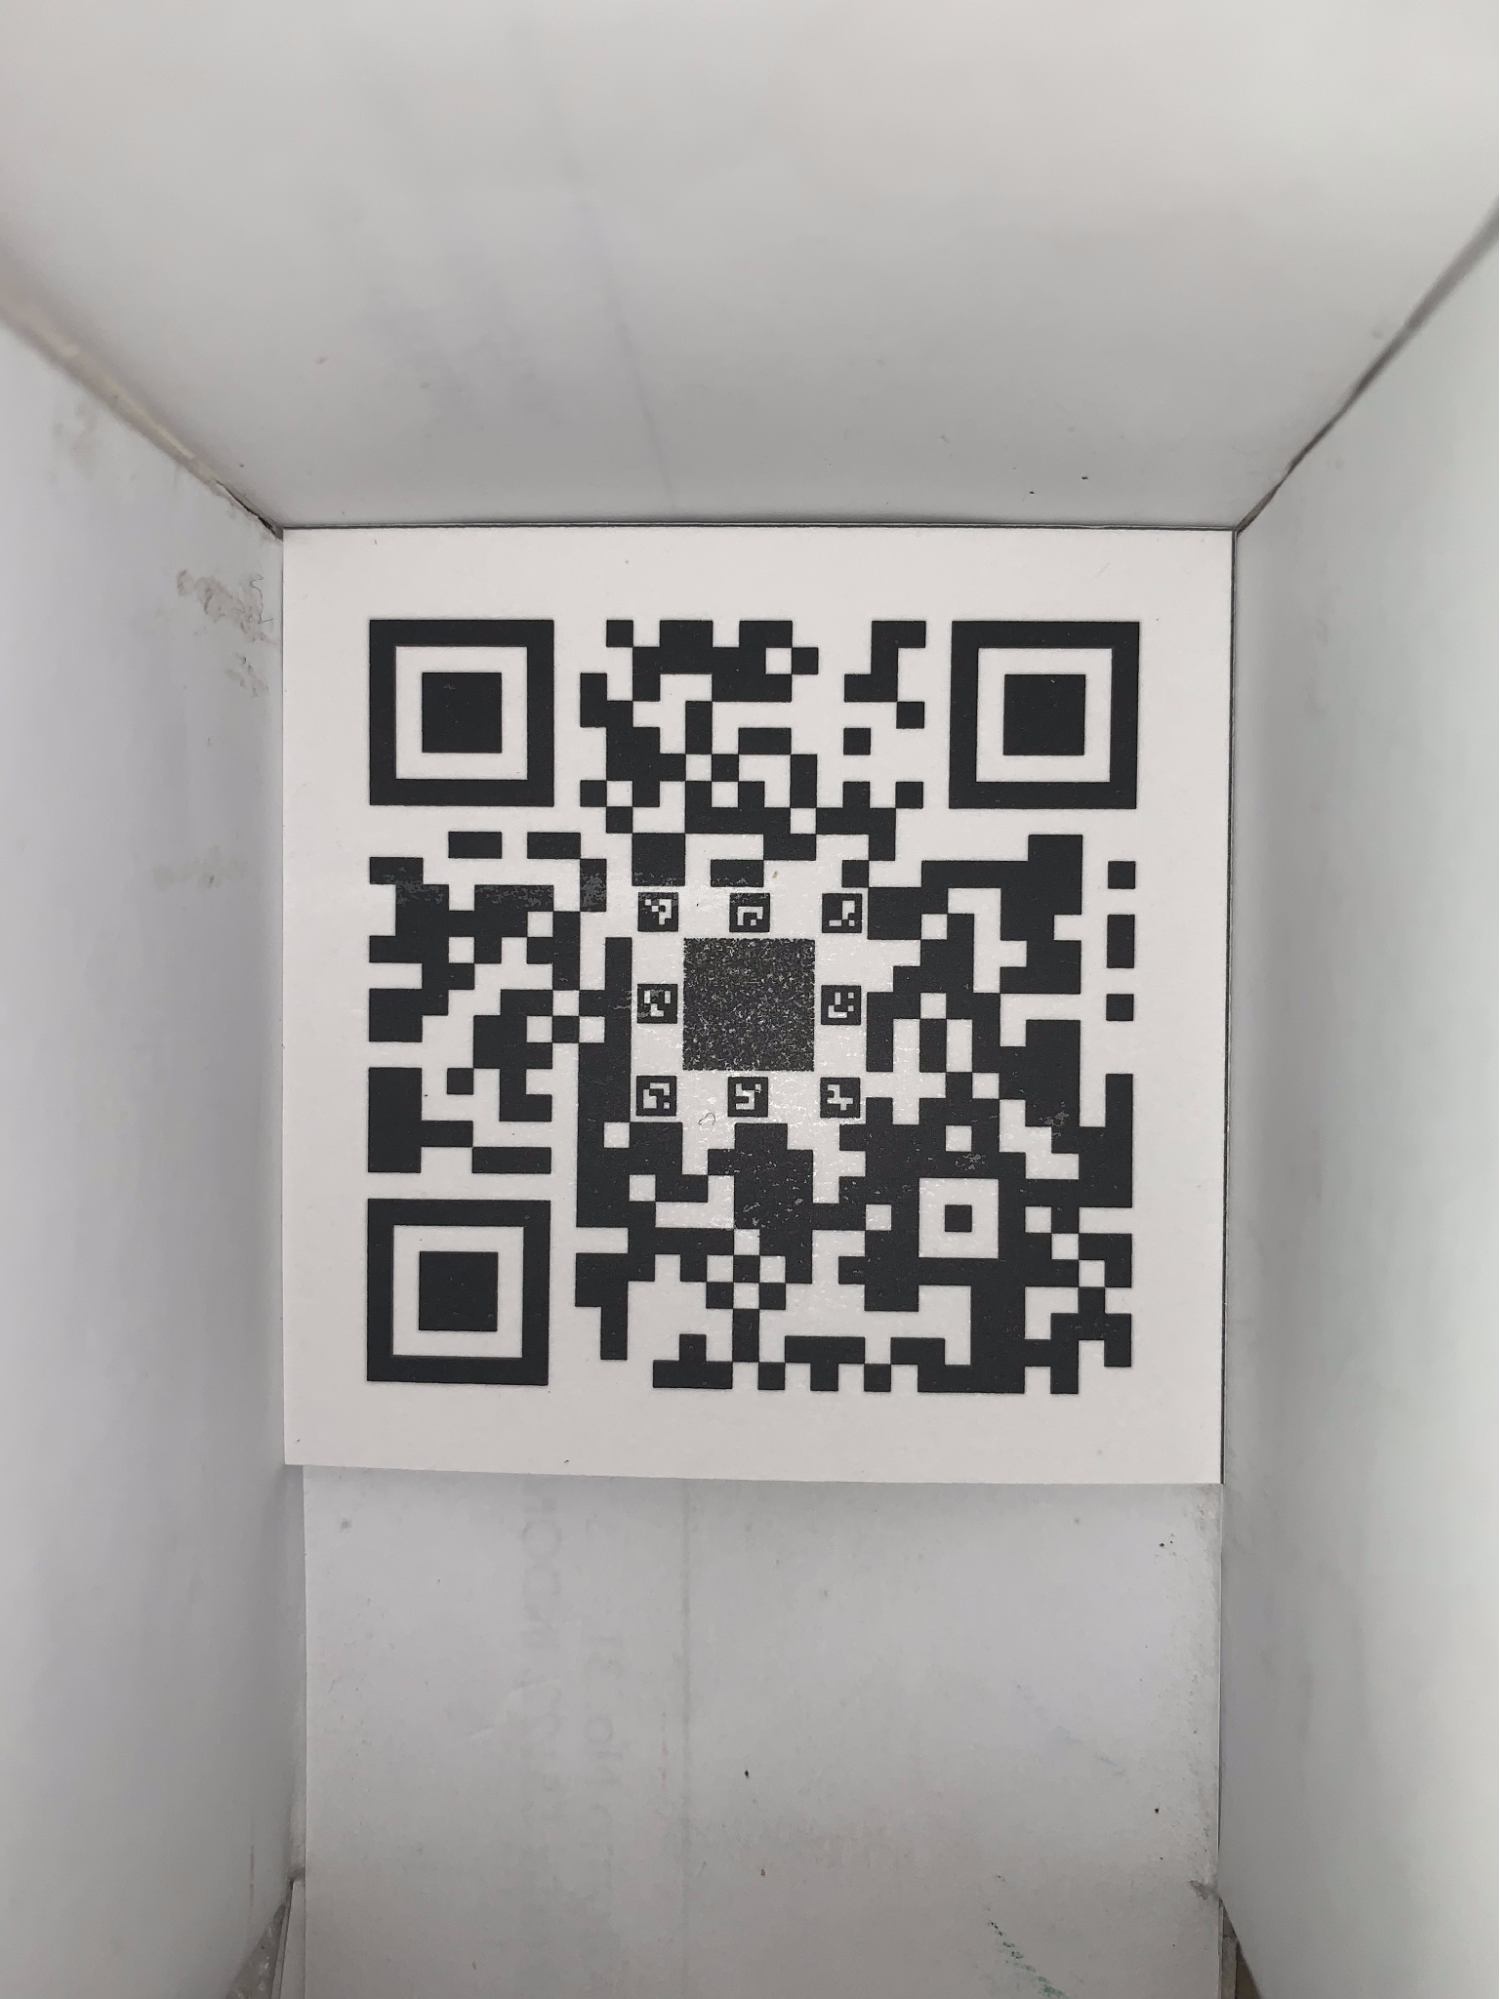
\includegraphics[width=7.5cm]{contents/chapter-4/4-hasilfotoiphonexr.png}
	\caption{Hasil pemotretan SQR menggunakan perangkat Iphone XR}
	\label{Fig: 4-hasilfotoiphonexr}
\end{figure}

\subsection{Jenis Kertas dan Tinta}
Jenis kertas dan tinta yang digunakan dalam pencetakan \emph{dataset} yang penulis gunakan adalah kertas bersifat \emph{doff}, sehingga tidak memantulkan
cahaya dari \emph{flash smarthpone} saat pemotretan berlangsung. Kertas bersifat \emph{doff} yang dapat digunakan seperti \emph{art carton} atau HVS. Opsi lain
adalah dapat menggunakan kertas dan tinta yang bersifat \emph{glossy}, namun diberikan laminasi \emph{doff} di akhir. Pada Gambar \ref{Fig:
	4-perbandingankertas}, dapat dilihat perbedaan hasil pemotretan menggunakan kertas \emph{doff} dan \emph{glossy}, SQR yang dicetak menggunakan kertas dan tinta
\emph{glossy} seperti \emph{ivory} akan memantulkan cahaya, SQR yang dicetak menggunakan kertas dan tinta \emph{doff} seperti \emph{art carton} akan terjaga
kualitasnya karena tidak terkena pantulan cahaya, sedangkan SQR yang dicetak menggunakan kertas dan tinta \emph{glossy} kemudian dilaminasi \emph{doff},
hasilnya baik, namun ada sedikit derau gelembung yang disebabkan oleh proses laminasi.

\begin{figure}[h]
	\centering
	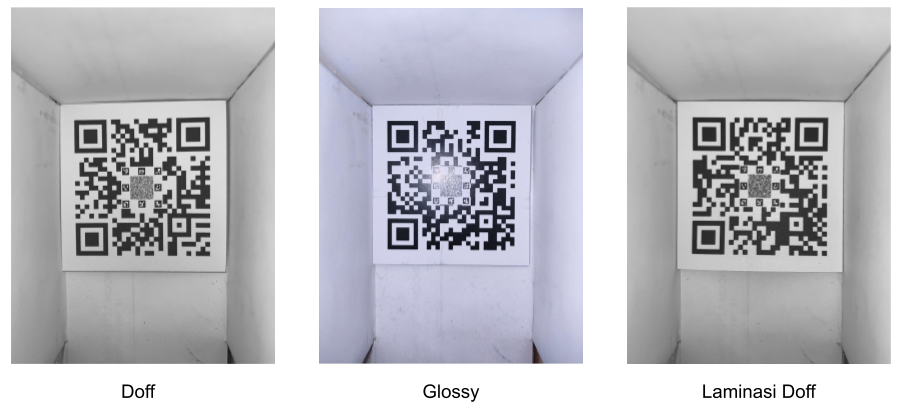
\includegraphics[width=15cm]{contents/chapter-4/4-perbandingankertas.png}
	\caption{Perbandingan gambar hasil pemotretan SQR yang dicetak dengan berbagai tipe kertas}
	\label{Fig: 4-perbandingankertas}
\end{figure}

\section{Hasil Pendeteksian Penanda ArUco}

\begin{table}[h]
	\caption{Tabel hasil pendeteksian penanda ArUco dengan berbagai ukuran}
	\vspace{0.5em}
	\centering
	\begin{tabular}{|c|c|c|}
		\hline
		\textbf{Ukuran ArUco} & \textbf{Jumlah Sukses Terdeteksi} & \textbf{Faktor Penskalaan Terkecil} \\
		\hline
		20                    & 0                                 & -                                   \\
		22                    & 1                                 & 0.3                                 \\
		24                    & 4                                 & 1                                   \\
		26                    & 3                                 & 0.7                                 \\
		28                    & 5                                 & 1                                   \\
		30                    & 5                                 & 1                                   \\
		32                    & 5                                 & 1                                   \\
		34                    & 5                                 & 1                                   \\ \hline
	\end{tabular}
	\label{Tab: 4-tabelhasildeteksiaruco}
\end{table}

Untuk mendapatkan ukuran penanda ArUco yang optimal, penulis menggunakan data uji sejumlah 40 SQR, yang ukuran penanda ArUco-nya berbeda-beda tiap lima SQR,
dari ukuran 20 s.d. 34. Hasil yang didapatkan adalah penanda ArUco dengan ukuran 28 s.d. 34 sukses terdeteksi seluruhnya dengan faktor penskalaan 1, seperti
dapat dilihat pada Tabel \ref{Tab: 4-tabelhasildeteksiaruco}, artinya hasil gambar tidak perlu di-\emph{scaling} untuk mendapatkan hasil deteksi kedelapan
penanda ArUco. Namun, supaya ukuran penanda ArUco tidak terlalu besar, penulis memilih ukuran 28 dan 30 untuk diuji performanya lebih lanjut. Pengujian
selanjutnya adalah menggunakan 40 data untuk masing-masing penanda ArUco berukuran 28 dan 30.

\begin{table}[h]
	\caption{Tabel hasil pendeteksian penanda ArUco dengan berbagai ukuran}
	\vspace{0.5em}
	\centering
	\begin{tabular}{|c|c|c|}
		\hline
		\textbf{Ukuran ArUco} & \textbf{Jumlah Sukses Terdeteksi} & \textbf{Faktor Penskalaan Terkecil} \\
		\hline
		28                    & 40                                & 0.8                                 \\
		30                    & 40                                & 0.9                                 \\ \hline
	\end{tabular}
	\label{Tab: 4-tabelhasildeteksiaruco2}
\end{table}

Hasilnya, seperti dapat dilihat pada Tabel \ref{Tab: 4-tabelhasildeteksiaruco2}, baik penanda ArUco berukuran 28 ataupun 30, semuanya dapat terdeteksi. Karena
hasilnya sama baik, penulis akhirnya memutuskan untuk menggunakan ukuran penanda ArUco yang lebih kecil untuk menghemat ruang yang digunakan pada
\emph{watermark} berukuran 180x180 piksel.

\subsection{Parameter Akhir yang Digunakan}
\noindent Dari hasil verifikasi parameter, berikut adalah parameter pembuatan model SQR:

\begin{itemize}
	\item Ukuran SQR: 580 x 580 piksel
	\item Ukuran SQR beserta \emph{padding}: 720 x 720 piksel
	\item Ukuran \emph{watermark}: 180 x 180 piksel
	\item Ukuran CDP: 100 x 100 piksel
	\item Jumlah penanda ArUco: 8
	\item Ukuran penanda ArUco: 30 x 30 piksel
\end{itemize}

\noindent Untuk parameter P\&S adalah sebagai berikut:
\begin{itemize}
	\item ISO: 200
	\item \emph{Shutter speed}: 1/100
	\item Fokus: 0,00
	\item \emph{White balance}: 4000
	\item Jenis kertas: \emph{Art carton}
	\item Jenis tinta: Tinta buku
\end{itemize}

\section{Deskripsi \emph{Dataset}}
\emph{Dataset} yang digunakan dalam foto SQR sejumlah 400 data dengan rincian: 200 data SQR orisinal 4 level serta 200 data SQR palsu 4 level. \emph{Dataset} tersebut dipotret menggunakan parameter yang telah ditetapkan melalui eksperimen. SQR orisinal merupakan SQR yang dicetak dari format digitalnya, sedangkan SQR palsu di-\emph{generate} dengan menempelkan CDP hasil lokalisasi ke dalam \emph{template} digital kode QR. Contoh sampel data \emph{raw photo} sebelum diolah dapat dilihat pada Gambar \ref{Fig: 4-sampelfotoraw}.

\begin{figure}[!h]
	\centering
	\includegraphics[width=7.5cm]{contents/chapter-4/4-sampelfotoraw.png}
	\caption{Sampel data yang dipotret}
	\label{Fig: 4-sampelfotoraw}
\end{figure}

\section{Analisis Hasil Lokalisasi CDP}
Analisis yang dilakukan adalah mencari interpolasi penskalaan yang memberikan hasil paling mirip dengan \emph{template}, kemudian menganalisis perbandingan
hasil lokalisasi CDP yang menggunakan penanda ArUco (8 titik) dan tanpa menggunakan penanda ArUco (4 titik).
% , dan yang terakhir adalah menganalisis
% karakteristik CDP 2 dan 4 level berdasarkan fitur jarak yang di-\emph{generate}.
\subsection{Analisis Perbandingan Hasil Lokalisasi CDP Orisinal dengan Berbagai Interpolasi Penskalaan}
Sebelum membuat \emph{dataset} SQR palsu, penulis melakukan analisis terhadap \emph{dataset} CDP orisinal hasil lokalisasi. Salah satu analisis yang dilakukan
adalah mencari interpolasi penskalaan yang hasil rata-rata jaraknya dengan \emph{template} paling minimal. Dengan jarak paling kecil, berarti hasil dari
pengolahan data foto pertama dengan interpolasi penskalaan tersebut paling mirip dengan \emph{template}. Hal tersebut menjadi salah satu langkah penyerangan
paling sederhana terhadap CDP orisinal. Hasil rata-rata jarak CDP orisinal dengan template dari masing-masing interpolasi penskalaan dan koefisien jarak dapat
dilihat pada Tabel \ref{Tab: 4-jarakorisinalberbagaiinterpolasi}.

\begin{table}[!ht]
	\centering
	\caption{Hasil rata-rata jarak CDP orisinal dengan \emph{template} dari berbagai interpolasi penskalaan dan koefisien jarak}
	\vspace{0.5em}
	\resizebox{\textwidth}{!}{\begin{tabular}{|l|r|r|r|r|r|}
			\hline
			\multicolumn{1}{|c|}{}  & \multicolumn{1}{c|}{\textbf{INTER\_NEAREST}} & \multicolumn{1}{c|}{\textbf{INTER\_LINEAR}} & \multicolumn{1}{c|}{\textbf{INTER\_AREA}} & \multicolumn{1}{c|}{\textbf{INTER\_CUBIC}} & \multicolumn{1}{c|}{\textbf{INTER\_LANCZOS4}} \\ \hline
			\textbf{sp\_corr}       & 0.8733                                       & \textbf{0.1558}                             & 0.219                                     & 0.1818                                     & 0.1969                                        \\ \hline
			\textbf{sp\_cosine}     & 0.5271                                       & \textbf{0.0708}                             & 0.1751                                    & 0.102                                      & 0.1117                                        \\ \hline
			\textbf{sp\_euclidean}  & 0.7409                                       & \textbf{0.1242}                             & 0.4054                                    & 0.1998                                     & 0.2166                                        \\ \hline
			\textbf{sp\_canberra}   & 0.6098                                       & \textbf{0.1355}                             & 0.5022                                    & 0.239                                      & 0.2464                                        \\ \hline
			\textbf{his\_corr}      & 0.9097                                       & 0.7019                                      & 0.8851                                    & 0.6437                                     & \textbf{0.4568}                               \\ \hline
			\textbf{his\_cosine}    & 0.964                                        & 0.5308                                      & 0.9642                                    & 0.5391                                     & \textbf{0.461}                                \\ \hline
			\textbf{his\_euclidean} & 0.7835                                       & \textbf{0.1689}                             & 0.7843                                    & 0.2045                                     & 0.2023                                        \\ \hline
			\textbf{his\_canberra}  & 0.9329                                       & 0.6476                                      & 0.8123                                    & 0.2149                                     & \textbf{0.1765}                               \\ \hline
			\textbf{dct\_corr}      & 0.4504                                       & \textbf{0.058}                              & 0.1574                                    & 0.0846                                     & 0.0922                                        \\ \hline
			\textbf{dct\_cosine}    & 0.4502                                       & \textbf{0.058}                              & 0.1574                                    & 0.0846                                     & 0.0922                                        \\ \hline
			\textbf{dct\_euclidean} & 0.7326                                       & \textbf{0.1623}                             & 0.4169                                    & 0.2271                                     & 0.2408                                        \\ \hline
			\textbf{dct\_canberra}  & 0.7462                                       & \textbf{0.2985}                             & 0.3739                                    & 0.6722                                     & 0.7312                                        \\ \hline
		\end{tabular}}
	\label{Tab: 4-jarakorisinalberbagaiinterpolasi}
\end{table}

\noindent Dari Tabel \ref{Tab: 4-jarakorisinalberbagaiinterpolasi}, terlihat bahwa interpolasi INTER\_LINEAR merupakan interpolasi penskalaan yang memiliki rata-rata jarak paling minimal, sedangkan INTER\_NEAREST memiliki jarak paling besar. Hal ini menunjukkan CDP hasil lokalisasi dengan interpolasi penskalaan INTER\_LINEAR paling mirip dengan \emph{template}.

Untuk hasil perbandingan secara visual hasil lokalisasi CDP menggunakan berbagai interpolasi penskalaan dapat dilihat pada Gambar x. Terlihat secara kasat mata
bahwa CDP yang dilokalisasi dengan interpolasi penskalaan INTER\_LINEAR memiliki hasil yang lebih mirip dengan \emph{template} dibandingkan dengan yang lain,
terutama CDP yang dilokalisasi dengan interpolasi penskalaan INTER\_NEAREST. Dari hasil tersebut, penulis memutuskan untuk menggunakan interpolasi penskalaan
INTER\_LINEAR dalam pembuatan pemrosesan CDP dan pembuatan \emph{dataset} selanjutnya.

\subsection{Analisis Perbandingan Hasil Lokalisasi CDP menggunakan Penanda ArUco dan Tanpa Penanda ArUco}
Analisis selanjutnya adalah membandingkan hasil lokalisasi CDP menggunakan delapan titik acuan dan empat titik acuan. Delapan titik acuan di sini adalah
delapan penanda ArUco, sedangkan empat titik adalah keempat titik sudut dari kode QR. Analisis yang dilakukan adalah menggunakan koefisien jarak yang mengukur
jarak dari CDP hasil lokalisasi dengan \emph{template}. Hasil lokalisasi yang lebih baik adalah yang jaraknya dengan \emph{template} lebih kecil yang berarti
lebih mirip dengan \emph{template}. Hipotesis awal dari penulis adalah hasil lokalisasi menggunakan 8 titik acuan akan lebih baik daripada 4 titik acuan,
terlebih SQR dipotret pada kondisi permukaan yang tidak rata atau ada lekukan pada sisi-sisi SQR. Koefisien jarak yang digunakan untuk mengukur
kemiripan adalah koefisien jarak korelasi, kosinus, dan \emph{euclidean} dari fitur spasial. Pengujian dilakukan pada \emph{dataset} SQR orisinal dan palsu 4
level. Perbandingan yang dilakukan adalah berdasarkan rata-rata nilai jarak dari grup data.

\begin{table}[!ht]
	\centering
	\caption{Hasil perbandingan rata-rata jarak hasil lokalisasi 8 titik dan 4 titik pada \emph{dataset} CDP orisinal 4 level}
	\vspace{0.5em}
	\begin{tabular}{|l|r|r|}
		\hline
		                       & \multicolumn{1}{c|}{\textbf{8 Titik}} & \multicolumn{1}{c|}{\textbf{4 Titik}} \\ \hline
		\textbf{sp\_corr}      & \textbf{0.3994}                       & 0.8153                                \\ \hline
		\textbf{sp\_cosine}    & \textbf{0.1113}                       & 0.1347                                \\ \hline
		\textbf{sp\_euclidean} & \textbf{27474}                        & 28092                                 \\ \hline
	\end{tabular}
	\label{Tab: 4-jaraklokalisasiarucovsnonarucoori}
\end{table}

Hasil pada data CDP orisinal seperti yang terlihat pada Tabel \ref{Tab: 4-jaraklokalisasiarucovsnonarucoori} menunjukkan bahwa CDP yang dilokalisasi
menggunakan delapan penanda ArUco atau 8 titik memiliki hasil jarak yang lebih kecil. Hal ini menunjukkan bahwa pada data CDP orisinal, lokalisasi menggunakan
8 titik lebih baik daripada 4 titik dalam hal kemiripannya dengan \emph{template}.

\begin{table}[!ht]
	\centering
	\caption{Hasil perbandingan rata-rata jarak hasil lokalisasi 8 titik dan 4 titik pada \emph{dataset} CDP palsu 4 level}
	\vspace{0.5em}
	\begin{tabular}{|l|r|r|}
		\hline
		                       & \multicolumn{1}{l|}{\textbf{8 titik}} & \multicolumn{1}{l|}{\textbf{4 titik}} \\ \hline
		\textbf{sp\_corr}      & \textbf{0.6147}                       & 0.8749                                \\ \hline
		\textbf{sp\_cosine}    & \textbf{0.108}                        & 0.1382                                \\ \hline
		\textbf{sp\_euclidean} & \textbf{27797}                        & 29880                                 \\ \hline
	\end{tabular}
	\label{Tab: 4-jaraklokalisasiarucovsnonarucopalsu}
\end{table}

Hasil yang sama juga didapat pada CDP palsu, CDP yang dilokalisasi menggunakan delapan penanda ArUco atau 8 titik memiliki hasil jarak yang lebih kecil. Hal
ini menunjukkan bahwa pada data CDP palsu, lokalisasi menggunakan 8 titik lebih baik daripada 4 titik dalam hal kemiripannya dengan \emph{template}. Untuk
perbandingan visual salah satu hasil lokalisasi CDP menggunakan 4 titik dan 8 titik dapat dilihat pada Gambar \ref{Fig: 4-cdplokalisasi8vs4}. Terlihat bahwa
hasil lokalisasi CDP menggunakan 4 titik kurang rapi, ada celah kosong di atasnya yang bukan merupakan komponen CDP itu sendiri. Selain itu, hasil lokalisasi
CDP menggunakan 4 titik terlihat lebih kabur. Hal tersebut dapat disebabkan ada lekukan pada data SQR yang dipotret. Hasil lokalisasi CDP menggunakan 8
titik terlihat jauh lebih rapi pada perbandingan tersebut.

\begin{figure}[h]
	\centering
	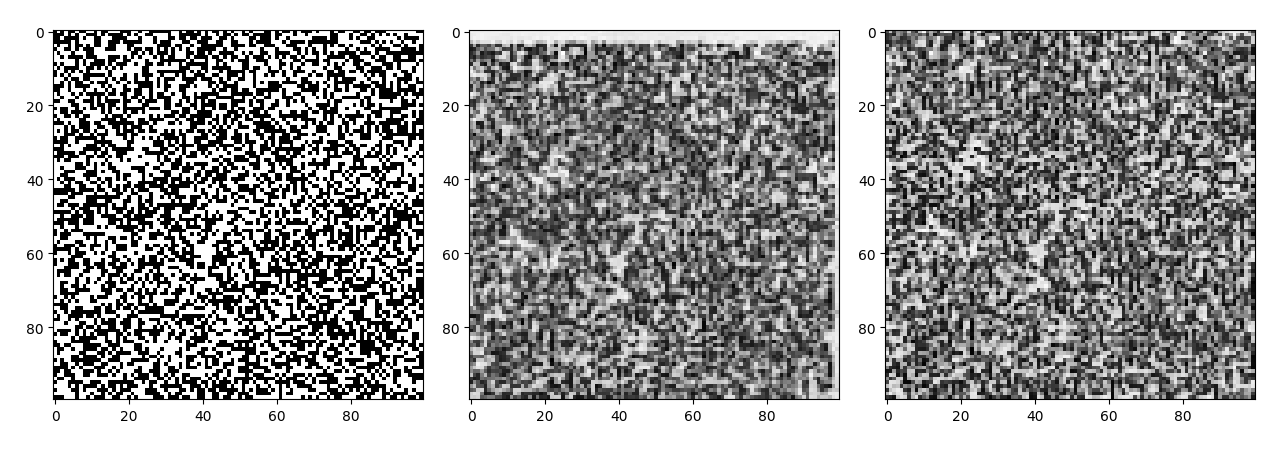
\includegraphics[width=12cm]{contents/chapter-4/4-cdplokalisasi8vs4_2.png}
	\caption{Perbandingan CDP \emph{template} dengan yang dilokalisasi dengan 4 titik (tengah) dan CDP yang dilokalisasi dengan 8 titik (kanan)}
	\label{Fig: 4-cdplokalisasi8vs4}
\end{figure}

Dari kedua pengujian pada CDP orisinal dan CDP palsu, dapat disimpulkan bahwa lokalisasi CDP menggunakan delapan penanda ArUco menghasilkan hasil lokalisasi
yang lebih baik dalam hal kemiripannya dengan \emph{template}. Hal tersebut tentunya akan berpengaruh dalam akurasi model yang akan dibuat, karena data CDP
yang diproses lebih berkualitas.

% \subsection{Perbandingan Hasil CDP \emph{Template}, Orisinal, dan Palsu}
% \subsection{Analisis Signifikansi CDP 2 dan 4 Level}
% \begin{table}[!h]
% 	\centering
% 	\caption{Hasil pengujian \emph{T-test} pada data grup fitur jarak CDP 2 level dengan data grup fitur jarak CDP 4 level}
% 	\vspace{0.5em}
% 	\begin{tabular}{|l|rr|rr|}
% 		\hline
% 		\multirow{2}{*}{}       & \multicolumn{2}{c|}{\textbf{Orisinal}}    & \multicolumn{2}{c|}{\textbf{Palsu}}                                                                                       \\ \cline{2-5}
% 		                        & \multicolumn{1}{c|}{\textbf{T-statistic}} & \multicolumn{1}{c|}{\textbf{P-value}} & \multicolumn{1}{c|}{\textbf{T-statistic}} & \multicolumn{1}{c|}{\textbf{P-value}} \\ \hline
% 		\textbf{sp\_corr}       & \multicolumn{1}{r|}{-16.7459}             & 5.01E-48                              & \multicolumn{1}{r|}{-15.4077}             & 2.42E-42                              \\ \hline
% 		\textbf{sp\_cosine}     & \multicolumn{1}{r|}{2.6649}               & 0.008014430587                        & \multicolumn{1}{r|}{5.6064}               & 3.87E-08                              \\ \hline
% 		\textbf{sp\_euclidean}  & \multicolumn{1}{r|}{18.6804}              & 2.27E-56                              & \multicolumn{1}{r|}{15.9246}              & 1.59E-44                              \\ \hline
% 		\textbf{sp\_canberra}   & \multicolumn{1}{r|}{13.5024}              & 1.81E-34                              & \multicolumn{1}{r|}{17.1141}              & 1.32E-49                              \\ \hline
% 		\textbf{his\_corr}      & \multicolumn{1}{r|}{34.4186}              & 2.31E-121                             & \multicolumn{1}{r|}{22.146}               & 2.13E-71                              \\ \hline
% 		\textbf{his\_cosine}    & \multicolumn{1}{r|}{77.323}               & 7.51E-242                             & \multicolumn{1}{r|}{69.1668}              & 6.46E-224                             \\ \hline
% 		\textbf{his\_euclidean} & \multicolumn{1}{r|}{43.2212}              & 2.09E-152                             & \multicolumn{1}{r|}{43.7259}              & 4.60E-154                             \\ \hline
% 		\textbf{his\_canberra}  & \multicolumn{1}{r|}{132.6975}             & 0                                     & \multicolumn{1}{r|}{88.0526}              & 4.52E-263                             \\ \hline
% 		\textbf{dct\_corr}      & \multicolumn{1}{r|}{4.2178}               & 3.06E-05                              & \multicolumn{1}{r|}{6.5174}               & 2.17E-10                              \\ \hline
% 		\textbf{dct\_cosine}    & \multicolumn{1}{r|}{4.213}                & 3.12E-05                              & \multicolumn{1}{r|}{6.5082}               & 2.29E-10                              \\ \hline
% 		\textbf{dct\_euclidean} & \multicolumn{1}{r|}{14.0464}              & 1.10E-36                              & \multicolumn{1}{r|}{9.6896}               & 4.49E-20                              \\ \hline
% 		\textbf{dct\_canberra}  & \multicolumn{1}{r|}{-3.4369}              & 0.0006503627876                       & \multicolumn{1}{r|}{6.8627}               & 2.60E-11                              \\ \hline
% 	\end{tabular}
% 	\label{Tab: 4-hasilujisignifikansi2vs4level}
% \end{table}

% Analisis ini digunakan untuk mengetahui apakah ada perbedaan karakteristik yang mencolok antara CDP 2 dan 4 level, baik orisinal maupun palsu, diukur dari
% jaraknya dengan \emph{template}. Analisis dilakukan dengan melakukan uji statistik \emph{T-test} untuk menguji signifikansi antara data kelompok CDP orisinal 2
% dan 4 level dan juga CDP palsu 2 dan 4 level. Selain itu, dilakukan visualisasi plot distribusi untuk melihat secara visual karakteristik dan perbedaan dari
% kedua data grup berdasarkan jaraknya dengan \emph{template} untuk tiap-tiap koefisien jarak.

% Dari Tabel \ref{Tab: 4-hasilujisignifikansi2vs4level} terlihat bahwa hasilnya adalah signifikan untuk seluruh koefisien jarak, baik pada \emph{dataset} CDP
% orisinal dan palsu. Dua grup dapat dikatakan signifikan perbedaannya apabila memiliki \emph{P-value} < 0,05 (diambil dari nilai \emph{P-value} yang sering
% digunakan). Semakin kecil nilai \emph{P-value}, semakin signifikan perbedaan antara dua grup data. Dari Tabel \ref{Tab: 4-hasilujisignifikansi2vs4level} dapat
% dilihat bahwa koefisien jarak yang memiliki signifikansi tertinggi dalam membedakan kedua data grup adalah \emph{his\_canberra}, \emph{his\_cosine},
% \emph{his\_euclidean}, dan \emph{his\_corr}.

% Selain itu, untuk memudahkan melihat signifikansi antara kedua data grup secara visual, penulis melakukan plot distribusi untuk tiap-tiap koefisien jarak.
% Untuk hasil plot distribusi \emph{dataset} CDP orisinal dapat dilihat pada \ref{Fig: 4-ori2levelvsori4level}. Terlihat bahwa fitur histogram dapat memisahkan
% CDP 2 dan 4 level orisinal dengan baik. Hal ini sesuai dengan hasil pengujian statistik \emph{T-test} dengan empat peringkat teratas untuk jarak yang memiliki
% perbedaan paling signifikan, memisahkan 2 dan 4 level adalah \emph{his\_canberra}, \emph{his\_cosine}, \emph{his\_euclidean}, dan \emph{his\_corr}. Hasil lain
% yang diperoleh adalah CDP 4 level memiliki jarak yang lebih dekat dengan \emph{template} dibandingkan dengan CDP 2 level. Hal ini menunjukkan bahwa CDP 4 level
% lebih sulit terdegradasi melalui proses P\&S dibandingkan CDP 2 level.

% Selanjutnya untuk hasil plot distribusi \emph{dataset} CDP palsu dapat dilihat pada \ref{Fig: 4-fake2levelvsfake4level}. Terlihat bahwa hasilnya mirip bahkan
% hampir sama dengan plot distribusi pada \emph{dataset} CDP orisinal. Fitur histogram mampu memisahkan CDP 2 dan 4 level dengan baik. CDP 4 level juga memiliki
% jarak yang lebih dekat dengan \emph{template} dibandingkan dengan CDP 2 level. Analisis selanjutnya adalah melihat signifikansi antara CDP orisinal dan palsu
% berdasarkan fitur jaraknya.

% \clearpage

% \begin{figure}[!ht]
% 	\centering
% 	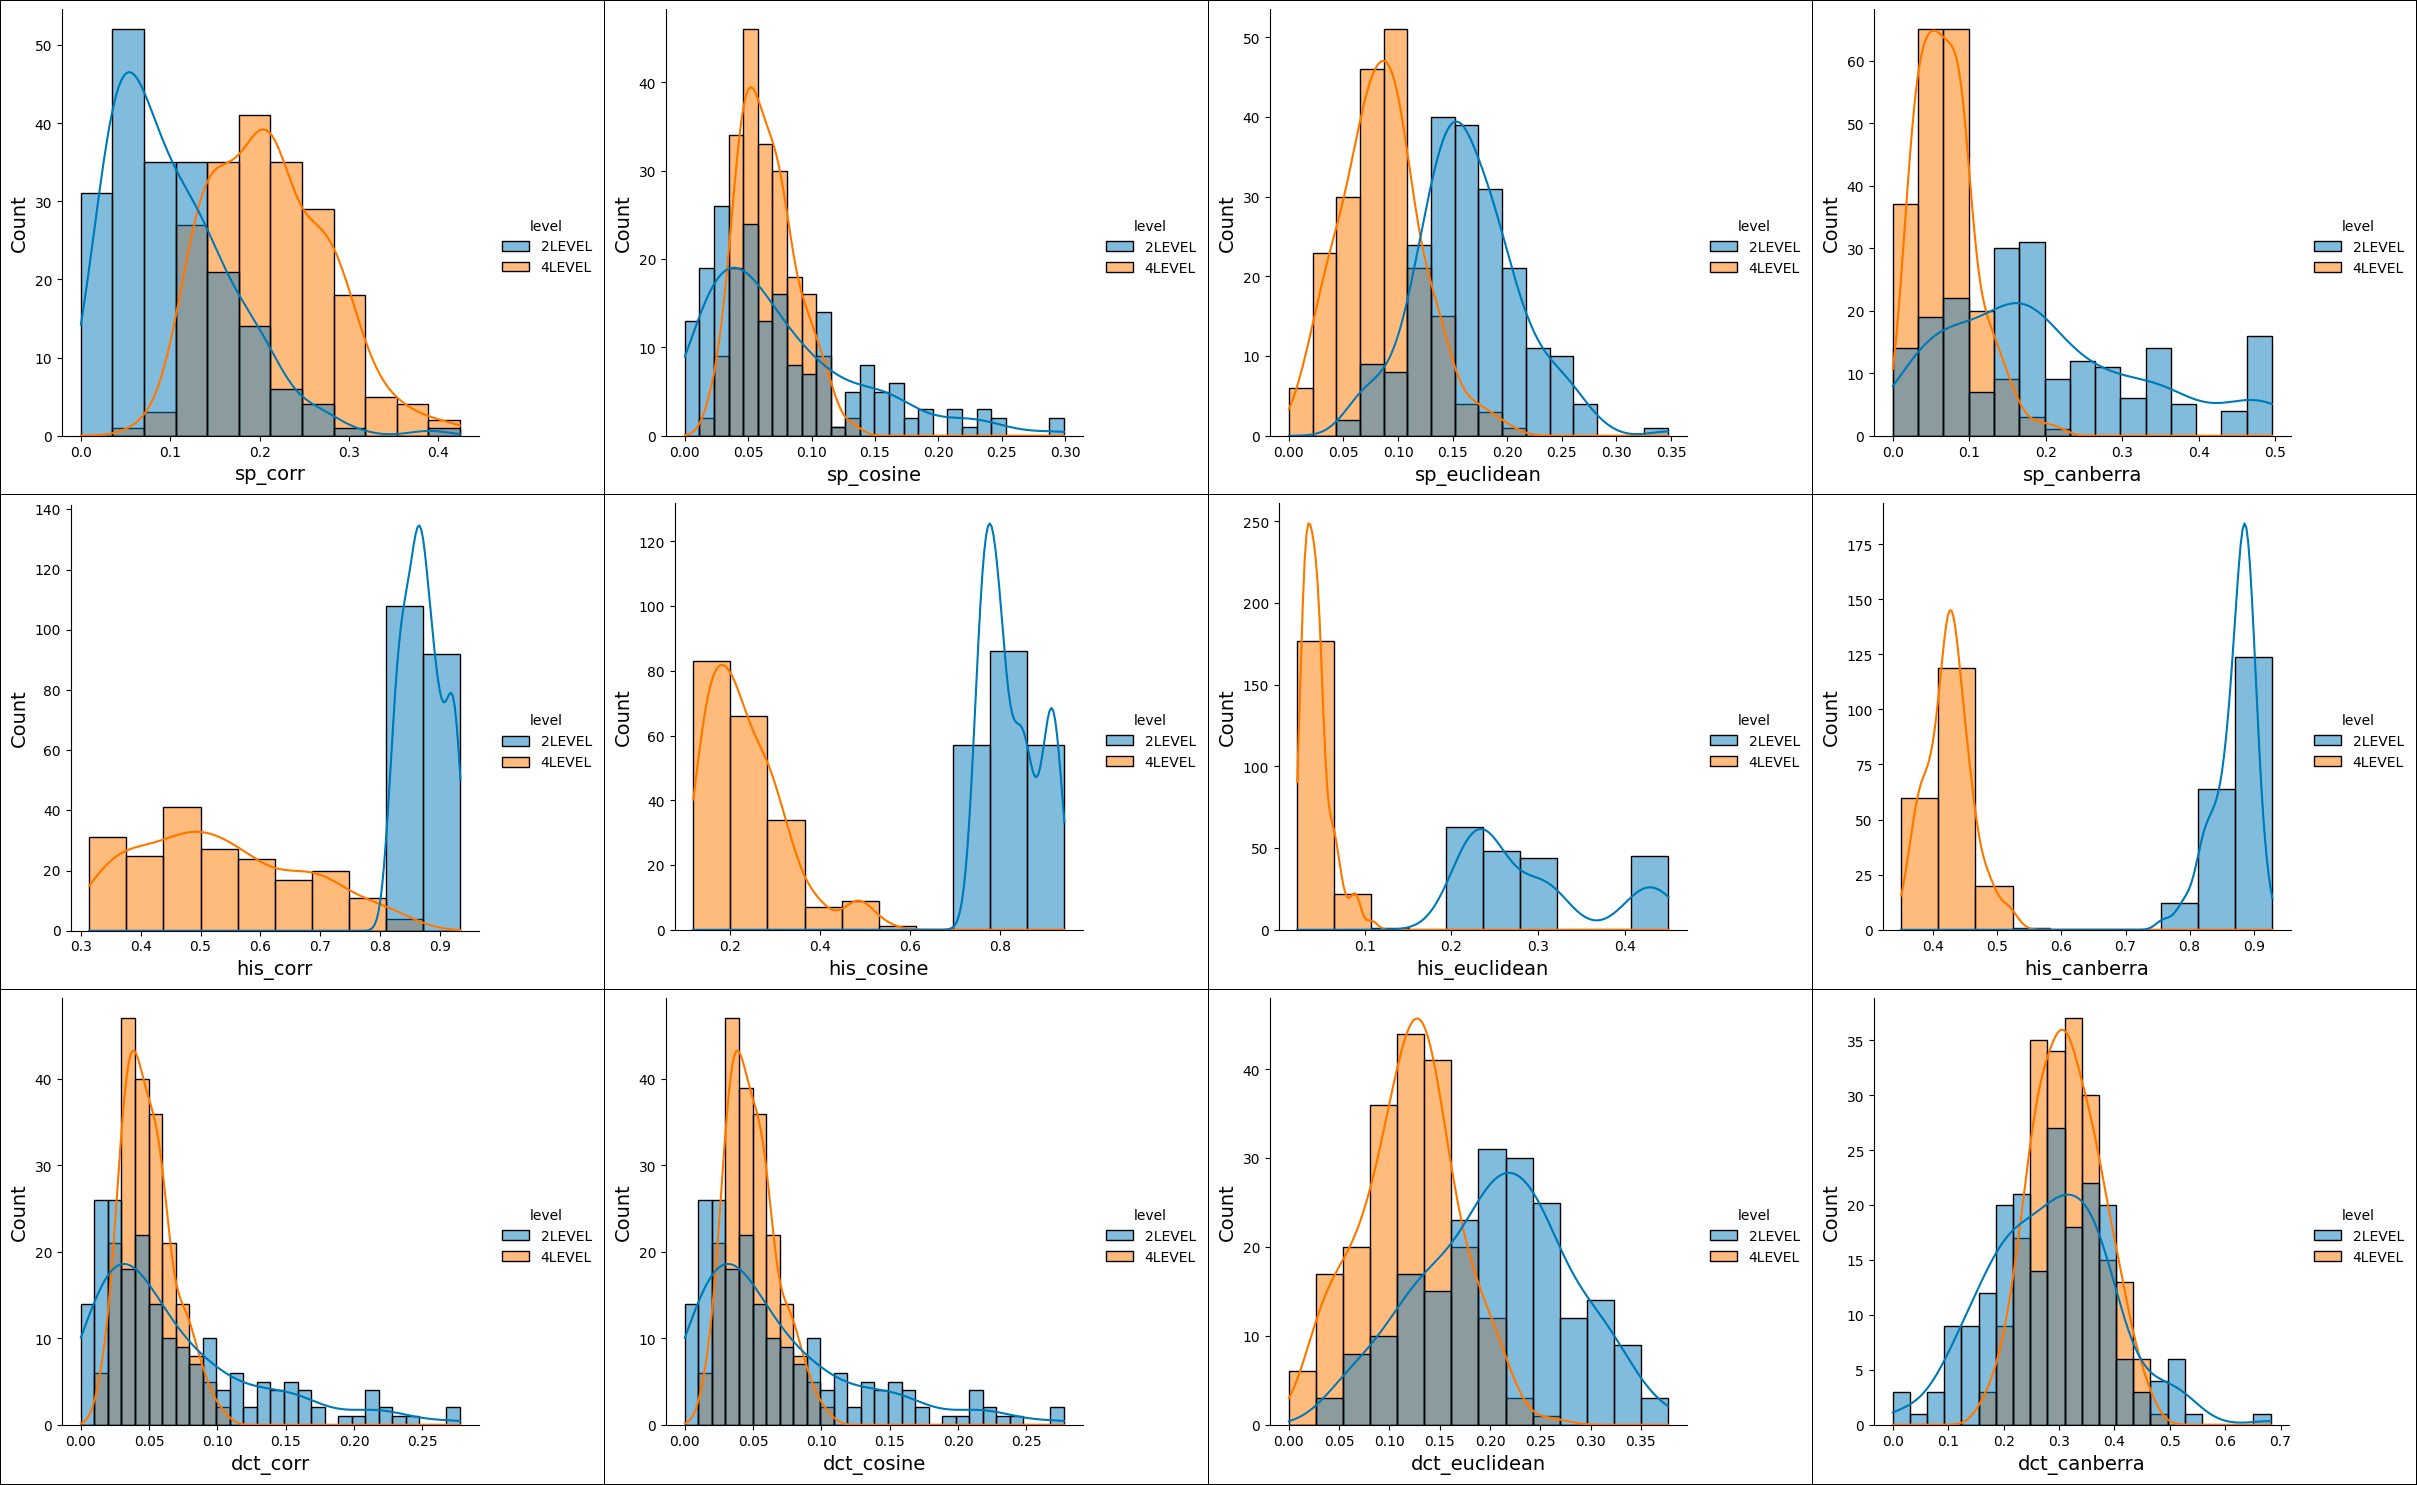
\includegraphics[width=\textwidth]{contents/chapter-4/4-ori2levelvsori4level.png}
% 	\caption{Plot distribusi koefisien jarak CDP orisinal 2 dan 4 level}
% 	\label{Fig: 4-ori2levelvsori4level}
% \end{figure}

% \begin{figure}[!ht]
% 	\centering
% 	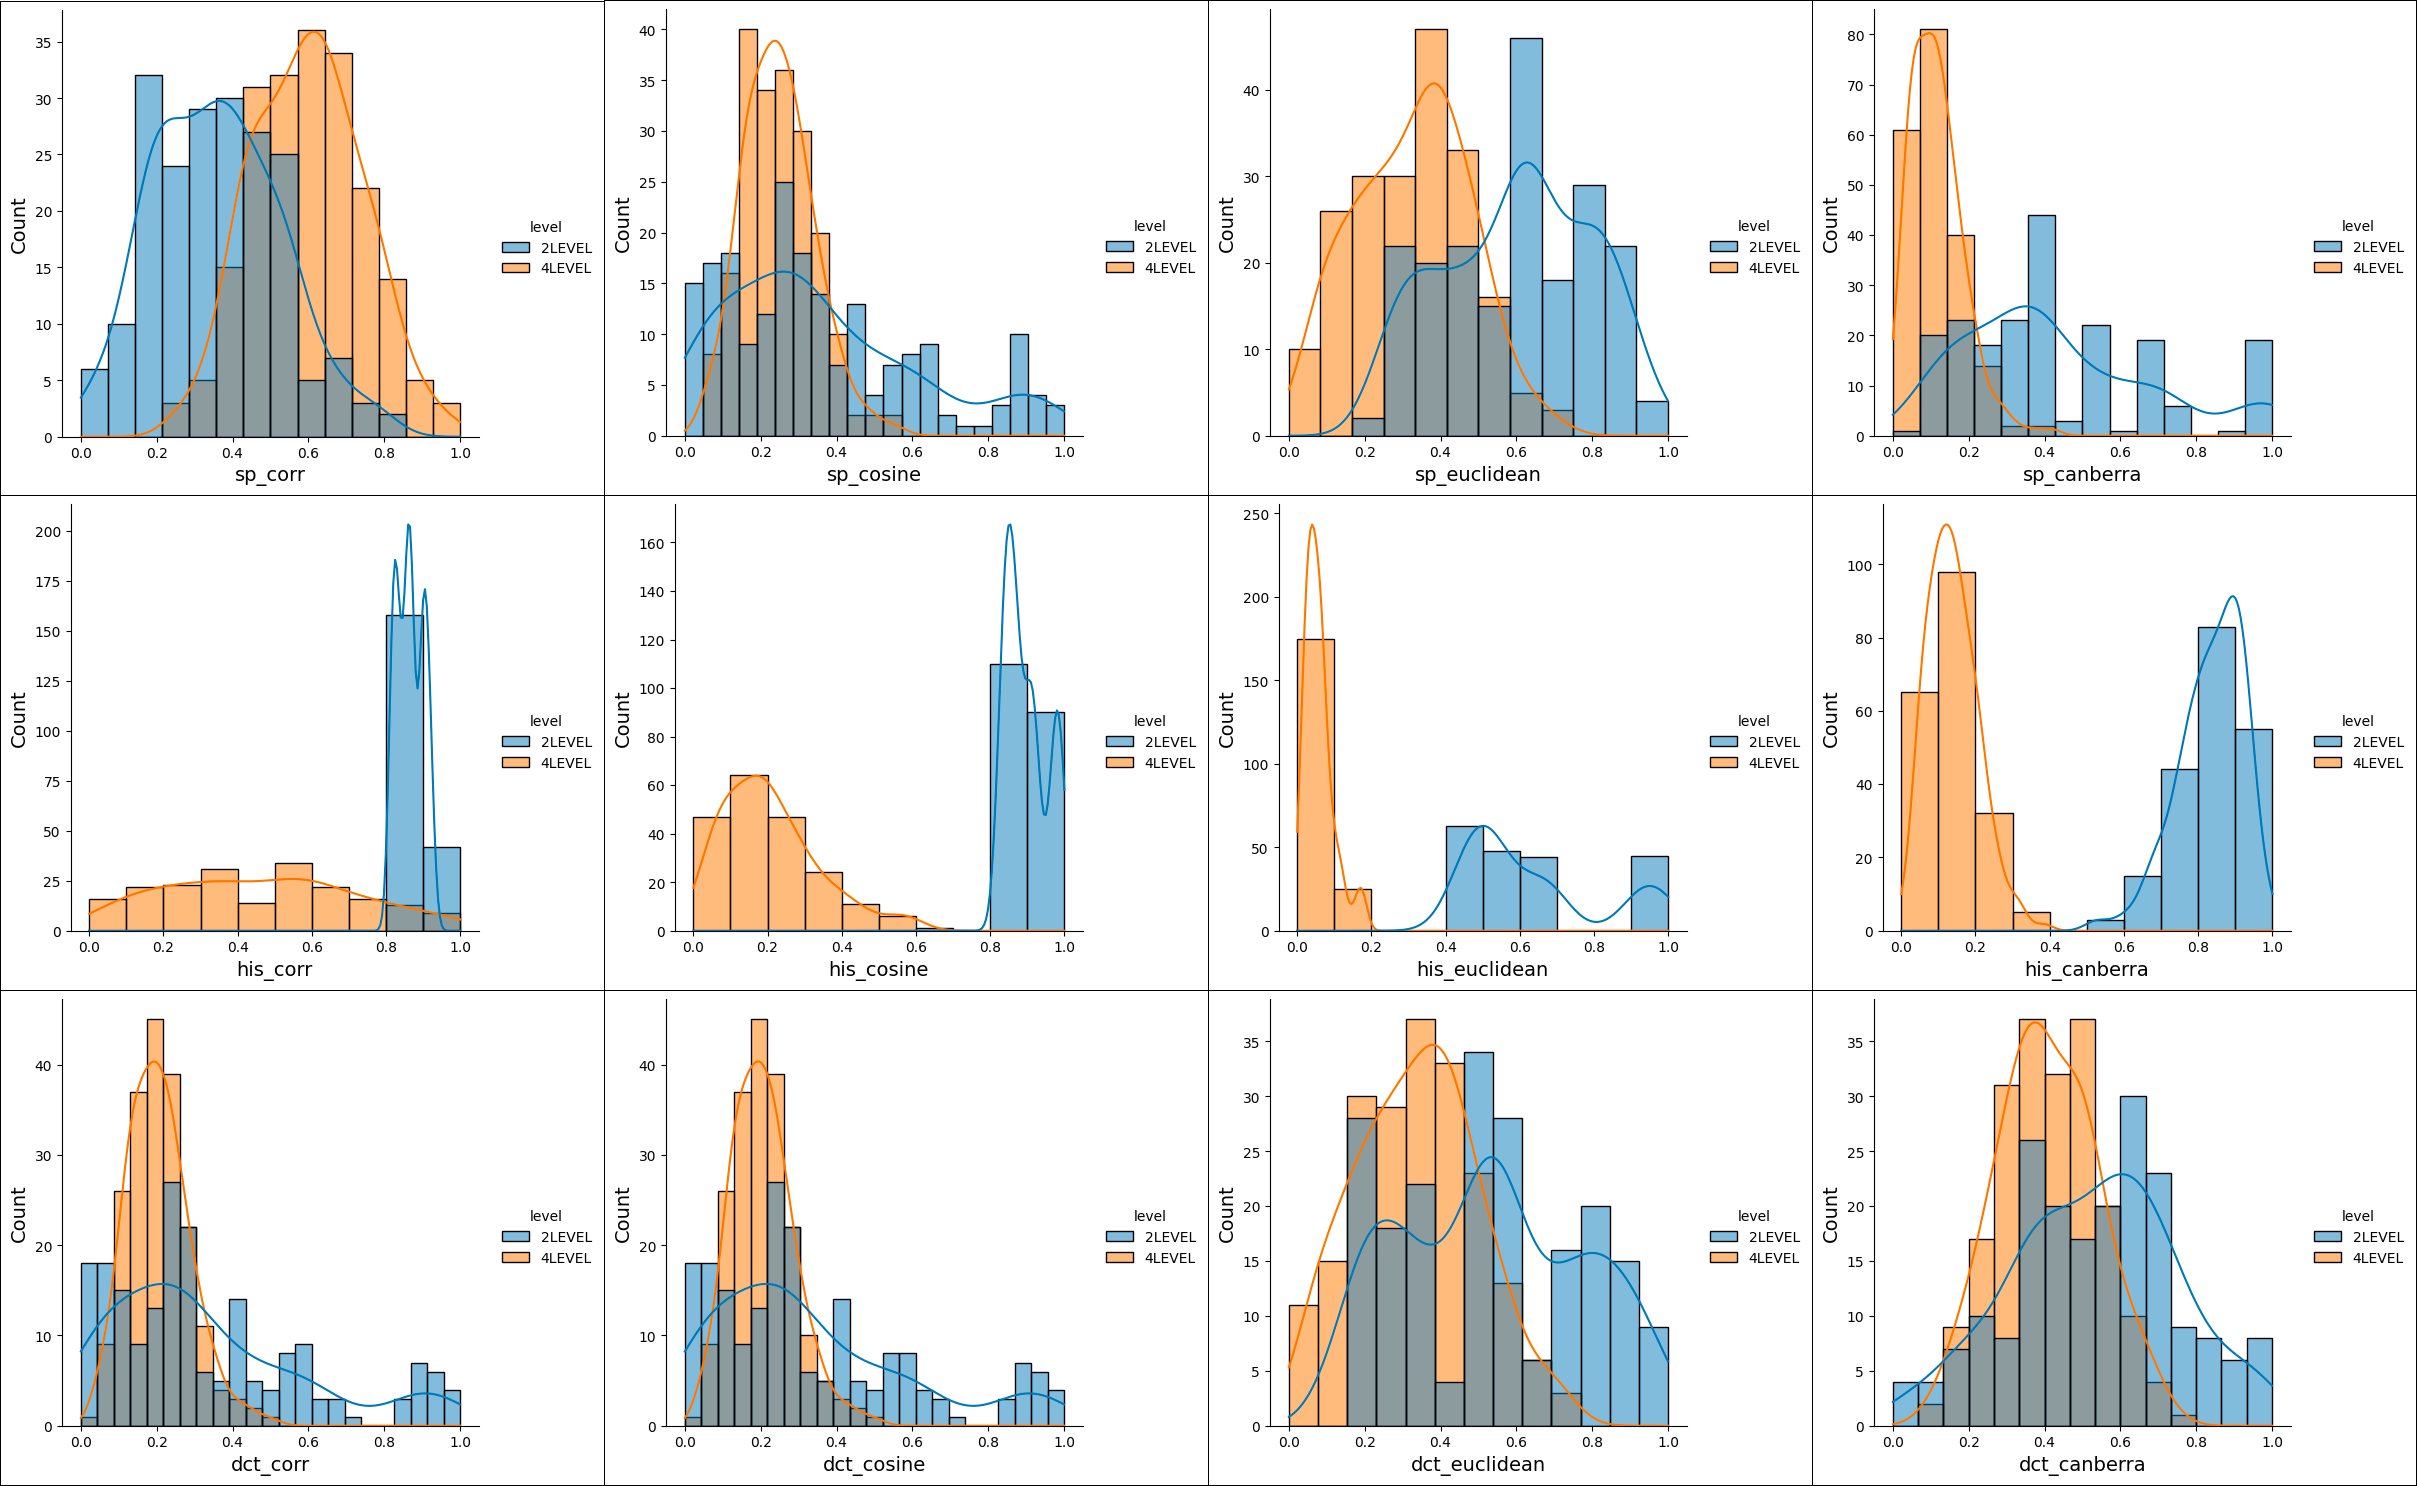
\includegraphics[width=\textwidth]{contents/chapter-4/4-fake2levelvsfake4level.png}
% 	\caption{Plot distribusi koefisien jarak CDP palsu 2 dan 4 level}
% 	\label{Fig: 4-fake2levelvsfake4level}
% \end{figure}

% \clearpage

\subsection{Analisis Signifikansi CDP Orisinal dan Palsu}
Analisis ini digunakan untuk mengetahui apakah ada perbedaan karakteristik yang mencolok antara CDP orisinal dan palsu, baik yang dilokalisasi menggunakan
penanda ArUco (8 titik) maupun yang dilokalisasi tanpa menggunakan penanda ArUco (4 titik). Analisis dilakukan dengan melakukan uji statistik \emph{T-test}
untuk menguji signifikansi antara data kelompok CDP orisinal dengan CDP palsu. Selain itu, dilakukan visualisasi plot distribusi untuk melihat secara visual
karakteristik dan perbedaan dari kedua data grup berdasarkan jaraknya dengan \emph{template} untuk tiap-tiap koefisien jarak.

% baik 2 level maupun 4 level, diukur dari jaraknya dengan \emph{template}. Analisis dilakukan dengan melakukan uji statistik \emph{T-test} untuk menguji
% signifikansi antara data kelompok CDP 2 level orisinal dan palsu dan juga CDP 4 level orisinal dan palsu. Selain itu, dilakukan visualisasi plot distribusi
% untuk melihat secara visual karakteristik dan perbedaan dari kedua data grup berdasarkan jaraknya dengan \emph{template} untuk tiap-tiap koefisien jarak.

\begin{table}[h]
	\centering
	\caption{Hasil pengujian \emph{T-test} pada data grup fitur jarak CDP orisinal dengan palsu, pada CDP yang dilokalisasi dengan 8 titik dan CDP yang dilokalisasi dengan 4 titik}
	\vspace{0.5em}
	\begin{tabular}{|l|rr|rr|}
		\hline
		\multirow{2}{*}{}       & \multicolumn{2}{c|}{\textbf{8 Titik}}     & \multicolumn{2}{c|}{\textbf{4 Titik}}                                                                                     \\ \cline{2-5}
		                        & \multicolumn{1}{c|}{\textbf{T-statistic}} & \multicolumn{1}{c|}{\textbf{P-value}} & \multicolumn{1}{c|}{\textbf{T-statistic}} & \multicolumn{1}{c|}{\textbf{P-value}} \\ \hline
		\textbf{sp\_corr}       & \multicolumn{1}{r|}{-56.5046}             & 3.32E-192                             & \multicolumn{1}{r|}{-4.3128}              & 2.04E-05                              \\ \hline
		\textbf{sp\_cosine}     & \multicolumn{1}{r|}{-32.3355}             & 2.08E-113                             & \multicolumn{1}{r|}{-0.8523}              & 0.3945606046                          \\ \hline
		\textbf{sp\_euclidean}  & \multicolumn{1}{r|}{-39.9488}             & 2.43E-141                             & \multicolumn{1}{r|}{-5.4538}              & 8.67E-08                              \\ \hline
		\textbf{sp\_canberra}   & \multicolumn{1}{r|}{-33.0441}             & 3.86E-116                             & \multicolumn{1}{r|}{-5.19}                & 3.36E-07                              \\ \hline
		\textbf{his\_corr}      & \multicolumn{1}{r|}{-6.0236}              & 3.89E-09                              & \multicolumn{1}{r|}{-6.0636}              & 3.10E-09                              \\ \hline
		\textbf{his\_cosine}    & \multicolumn{1}{r|}{-7.7801}              & 6.30E-14                              & \multicolumn{1}{r|}{-10.7008}             & 1.17E-23                              \\ \hline
		\textbf{his\_euclidean} & \multicolumn{1}{r|}{-6.6484}              & 9.79E-11                              & \multicolumn{1}{r|}{-11.2637}             & 9.84E-26                              \\ \hline
		\textbf{his\_canberra}  & \multicolumn{1}{r|}{-24.5923}             & 7.04E-82                              & \multicolumn{1}{r|}{-26.4865}             & 7.49E-90                              \\ \hline
		\textbf{dct\_corr}      & \multicolumn{1}{r|}{-29.4935}             & 3.53E-102                             & \multicolumn{1}{r|}{-1.2032}              & 0.2296019564                          \\ \hline
		\textbf{dct\_cosine}    & \multicolumn{1}{r|}{-29.5221}             & 2.71E-102                             & \multicolumn{1}{r|}{-1.2216}              & 0.2225752757                          \\ \hline
		\textbf{dct\_euclidean} & \multicolumn{1}{r|}{-29.7315}             & 3.90E-103                             & \multicolumn{1}{r|}{-8.8239}              & 3.53E-17                              \\ \hline
		\textbf{dct\_canberra}  & \multicolumn{1}{r|}{-55.4671}             & 2.32E-189                             & \multicolumn{1}{r|}{-7.6051}              & 2.07E-13                              \\ \hline
	\end{tabular}
	\label{Tab: 4-hasilujisignifikansiorivspalsu}
\end{table}

Dari Tabel \ref{Tab: 4-hasilujisignifikansiorivspalsu} terlihat bahwa dengan menggunakan nilai \emph{P-value} = 0,5, pada CDP yang dilokalisasi menggunakan 8
titik, seluruh fitur dapat dikatakan signifikan antara CDP orisinal dengan CDP palsunya. Namun, pada CDP yang dilokalisasi menggunakan 4 titik, ada yang
nilainya tidak signifikan, yaitu pada fitur jarak \emph{sp\_cosine}, \emph{dct\_corr}, dan \emph{dct\_cosine}. Selain itu, level signifikansinya juga berbeda
jauh antara CDP yang dilokalisasi dengan 8 titik dan CDP yang dilokalisasi dengan 4 titik. CDP yang dilokalisasi dengan 8 titik memiliki signifikansi yang jauh
lebih tinggi, terlihat dari kecilnya \emph{P-value} yang didapat pada masing-masing koefisien jarak.

% pada CDP 2 level, ada 2 fitur jarak yang
% tidak signifikan antara CDP orisinal dan palsunya, yaitu \emph{his\_corr} dan \emph{his\_euclidean}. Pada CDP 4 level, dengan nilai \emph{P-value} yang sama,
% seluruh fitur jarak dapat dikatakan signifikan antara CDP orisinal dan palsunya. Dari Tabel \ref{Tab: 4-hasilujisignifikansiorivspalsu} dapat dilihat bahwa
% baik CDP 2 dan 4 level, koefisien jarak yang memiliki nilai paling signifikan antara orisinal dan palsu adalah \emph{sp\_corr}, disusul \emph{dct\_canberra},
% dan \emph{sp\_euclidean}.

Selain itu, untuk memudahkan melihat signifikansi antara kedua data grup secara visual, penulis melakukan plot distribusi untuk tiap-tiap koefisien jarak.
Untuk hasil plot distribusi \emph{dataset} CDP yang dilokalisasi dengan 8 titik dan \emph{dataset} CDP yang dilokalisasi dengan 4 titik dapat dilihat pada
Gambar \ref{Fig: 4-4levelorivs4levelfake} dan \ref{Fig: 4-orivsfake4titik}. Hasilnya sangat terlihat bahwa pada \emph{dataset} CDP yang dilokalisasi dengan 8
titik, distribusi antara CDP orisinal dengan palsunya dapat terpisahkan dengan baik, sedangkan pada \emph{dataset} CDP yang dilokalisasi dengan 4 titik,
distribusi antara CDP orisinal dengan palsunya tidak terpisahkan dengan baik, terlihat dari banyaknya \emph{overlap}. Hal tersebut menunjukkan bahwa CDP yang
dilokalisasi dengan 8 titik mendapatkan fitur yang signifikansi antara CDP orisinal dengan palsunya sangat tinggi.

% CDP 2 level dapat dilihat pada \ref{Fig: 4-2levelorivs2levelfake}. Terlihat bahwa pada \emph{dataset} CDP 2 level,
% fitur terbaik yang memisahkan CDP orisinal dan palsu adalah \emph{sp\_corr}. Selain itu, fitur spasial yang lain juga memiliki signifikansi yang tinggi. Selain
% itu, ada fitur \emph{dct\_canberra} yang juga memiliki signifikansi yang tinggi.

% \begin{figure}[!h]
% 	\centering
% 	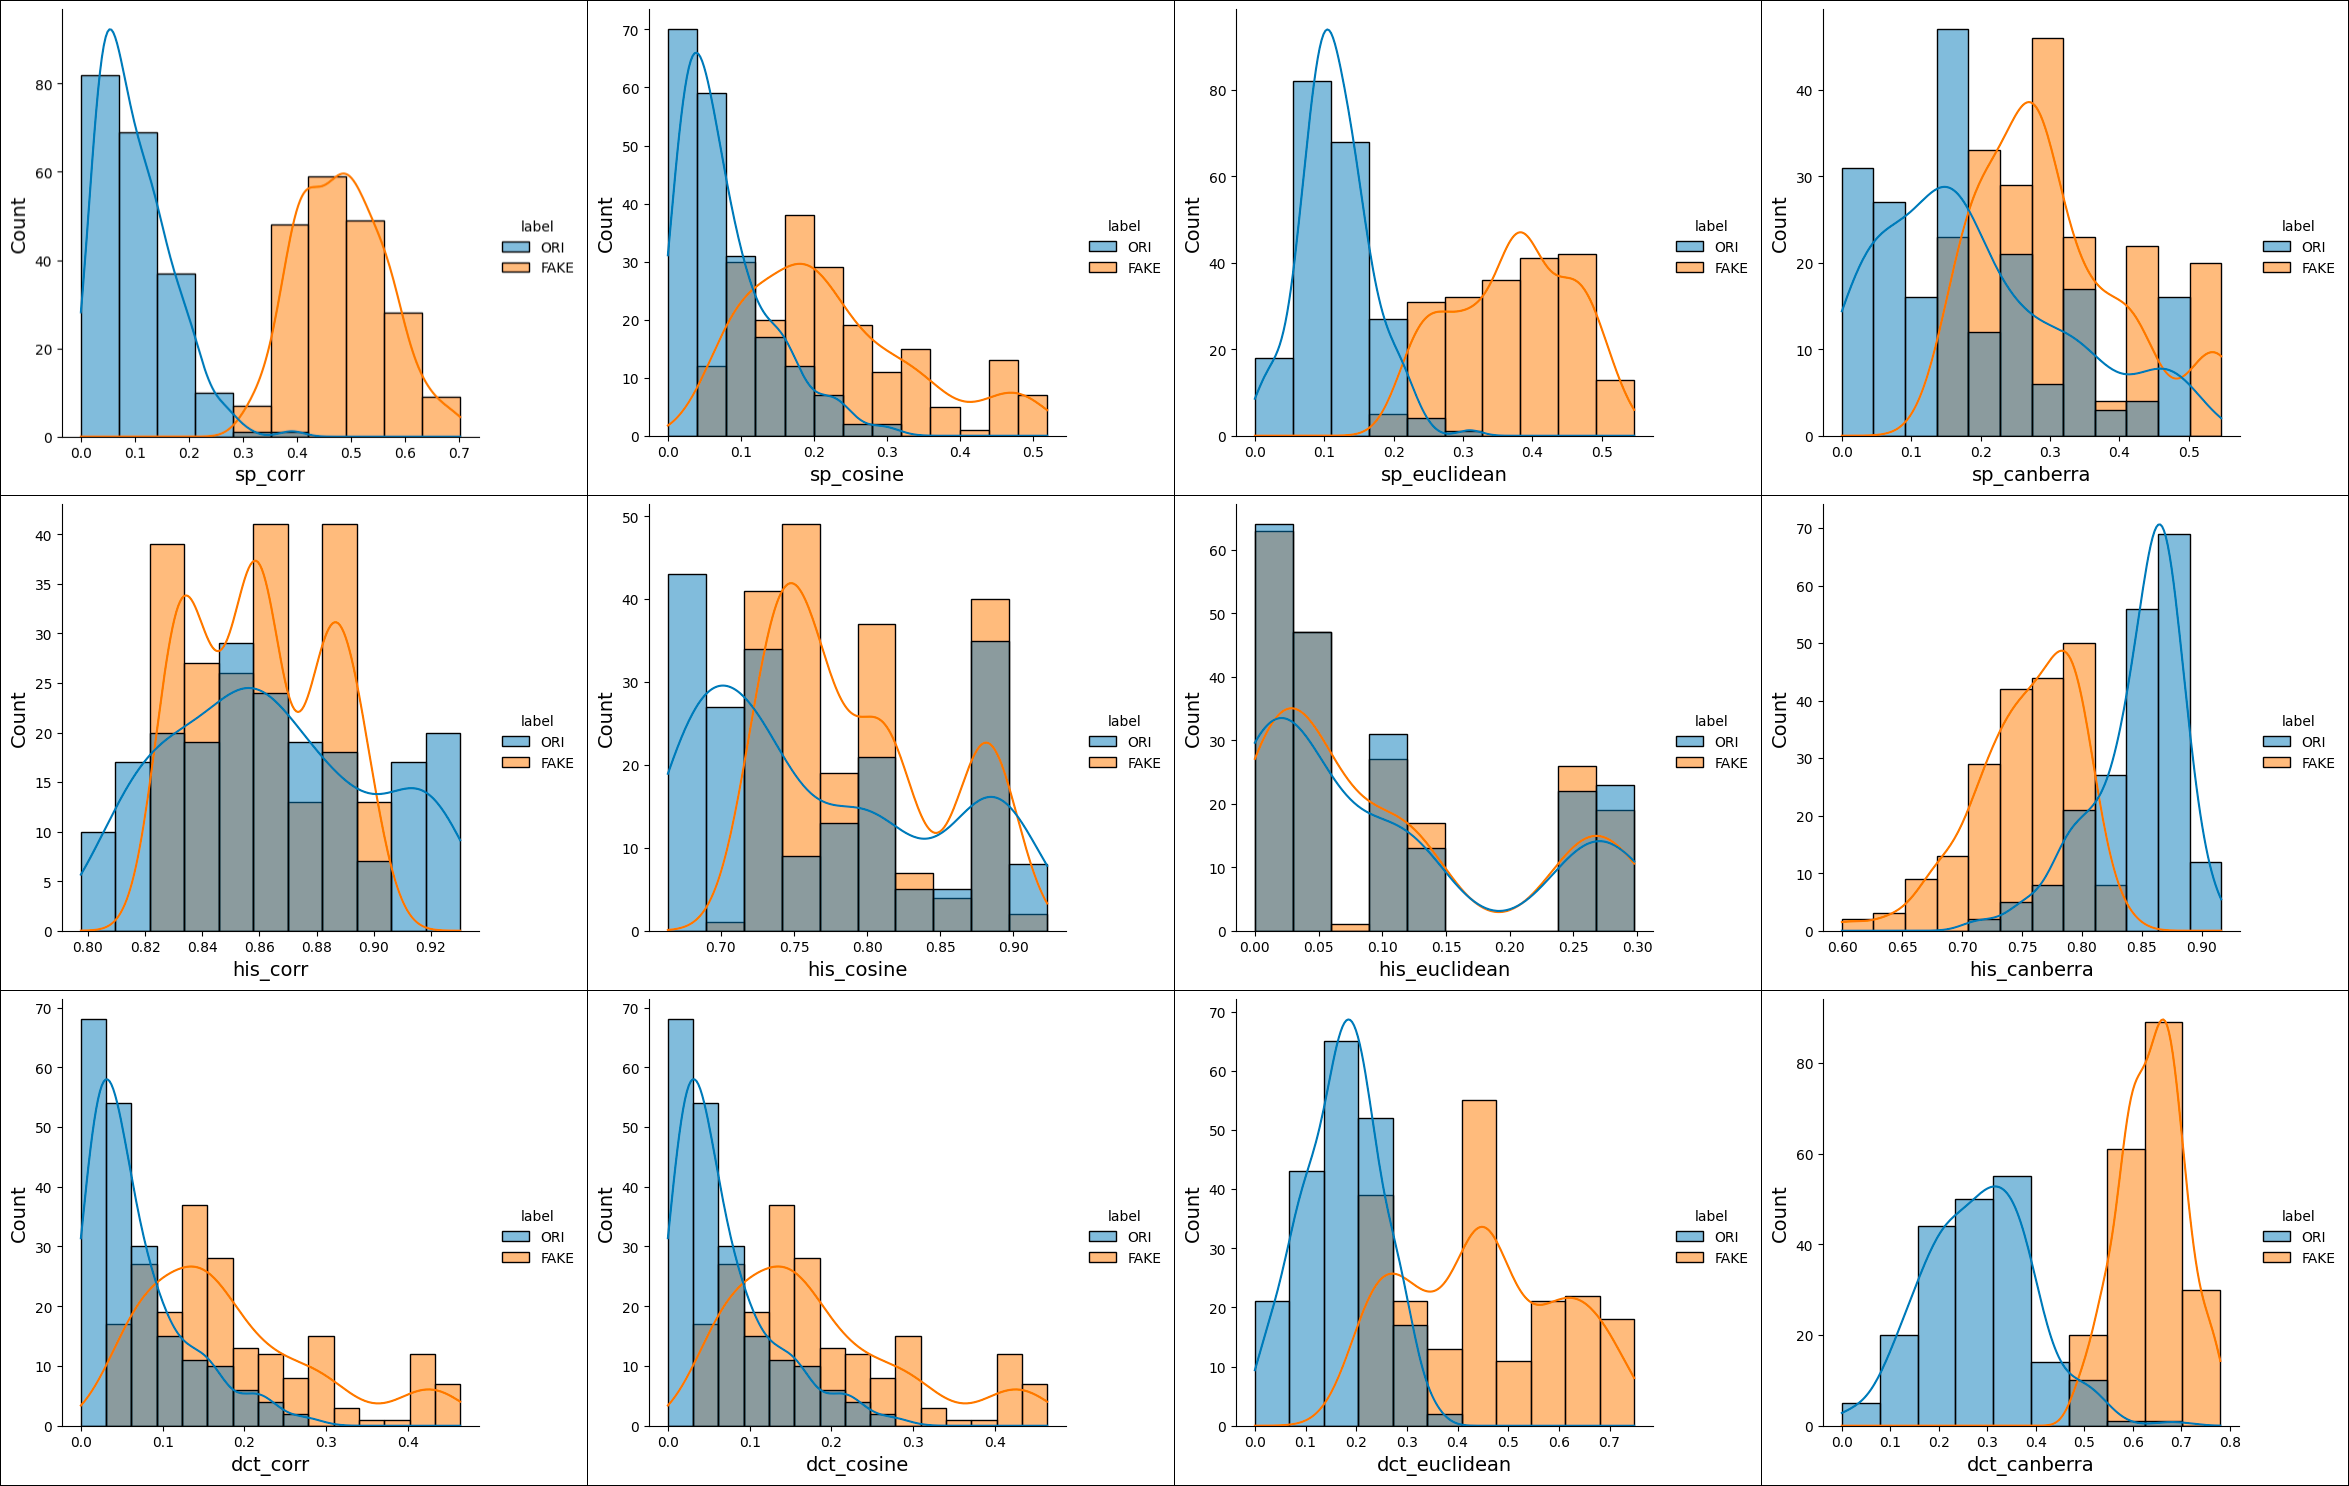
\includegraphics[width=\textwidth]{contents/chapter-4/4-2levelorivs2levelfake.png}
% 	\caption{Plot distribusi koefisien jarak CDP 2 level orisinal dan palsu}
% 	\label{Fig: 4-2levelorivs2levelfake}
% \end{figure}

\clearpage

\begin{figure}[!h]
	\centering
	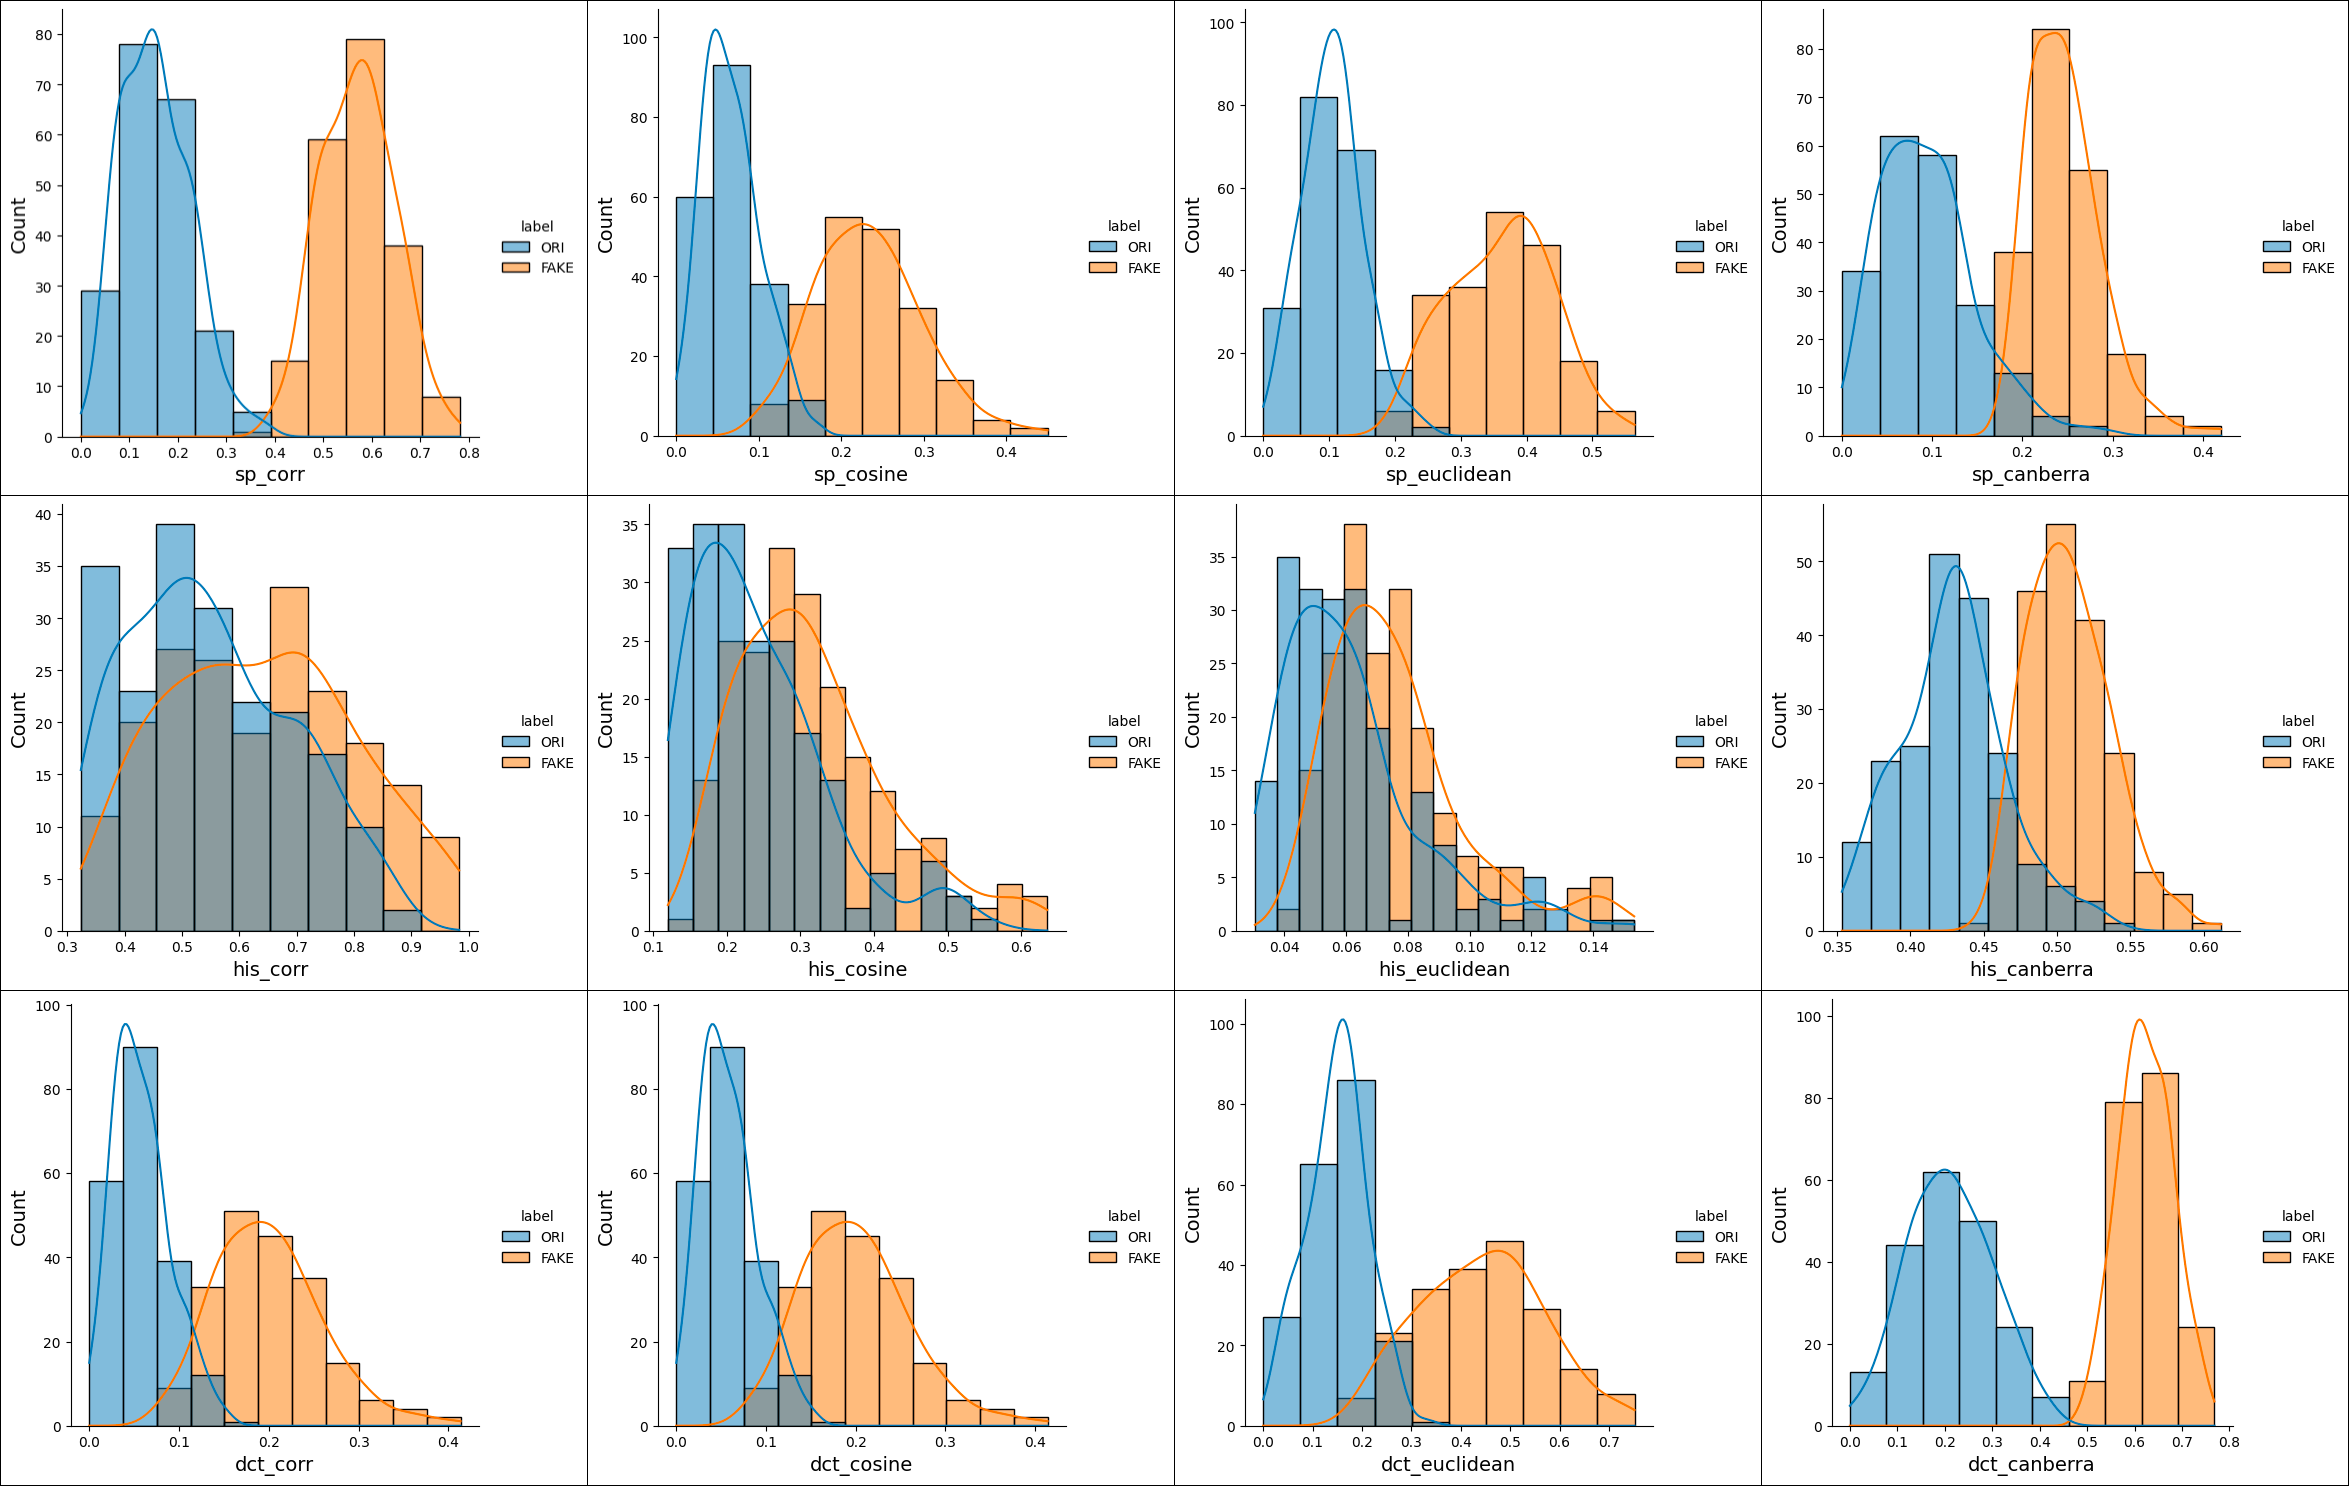
\includegraphics[width=\textwidth]{contents/chapter-4/4-4levelorivs4levelfake.png}
	\caption{Plot distribusi koefisien jarak pada CDP 4 level yang dilokalisasi dengan 8 titik}
	\label{Fig: 4-4levelorivs4levelfake}
\end{figure}

\begin{figure}[!h]
	\centering
	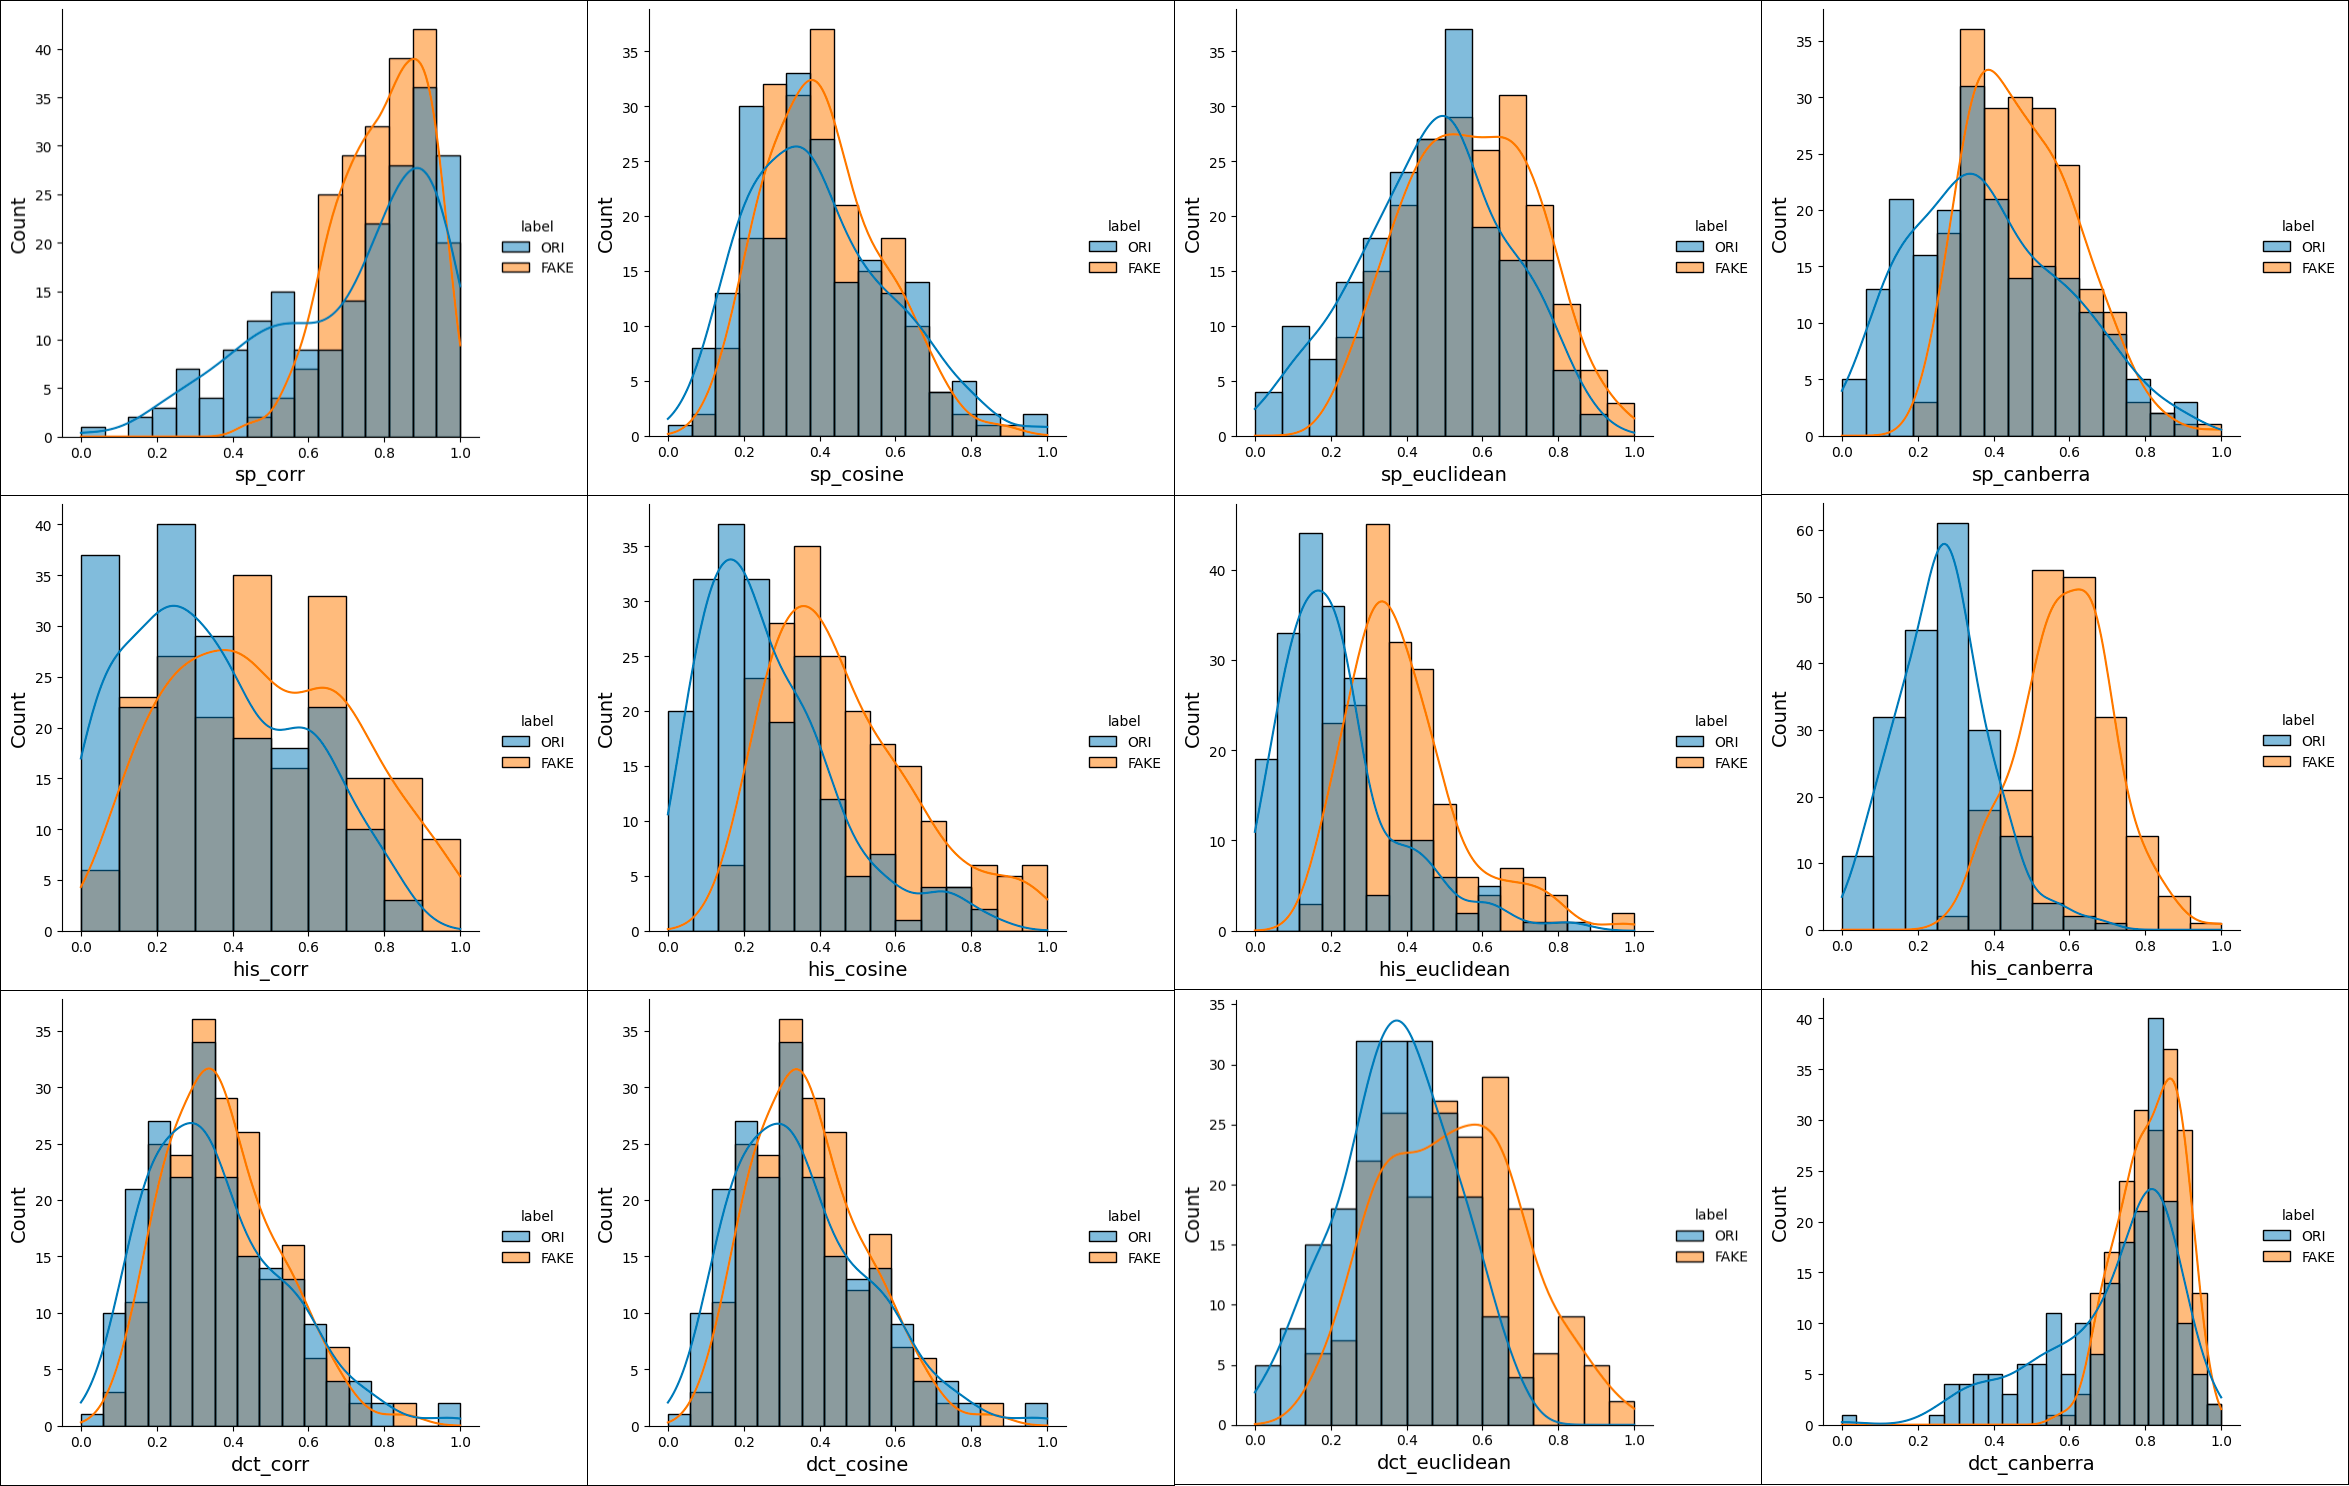
\includegraphics[width=\textwidth]{contents/chapter-4/4-orivsfake4titik.png}
	\caption{Plot distribusi koefisien jarak pada CDP 4 level yang dilokalisasi dengan 4 titik}
	\label{Fig: 4-orivsfake4titik}
\end{figure}

\clearpage

% Selanjutnya untuk hasil plot distribusi \emph{dataset} CDP 4 level dapat dilihat pada \ref{Fig: 4-4levelorivs4levelfake}. Terlihat bahwa hasilnya mirip bahkan
% hampir sama dengan plot distribusi pada \emph{dataset} CDP 2 level. Fitur \emph{sp\_corr} menjadi fitur paling baik yang memisahkan CDP orisinal dan palsu .
% Selain itu, fitur \emph{dct\_canberra} juga memiliki signifikansi yang tinggi. Secara umum analisis fitur jarak menghasilkan hasil yang baik, yaitu mayoritas
% fitur jarak mampu memisahkan CDP orisinal dan palsu, sehingga sangat mungkin hasil model klasifikasi biner yang dibuat memiliki tingkat akurasi yang tinggi
% karena fitur yang digunakan untuk pelatihan sangat berkualitas.

\section{Hasil Pemodelan Klasifikasi Biner}
Pemodelan dilakukan menggunakan dua metode, pertama menggunakan fitur tunggal dari tiap-tiap koefisien jarak, kedua menggunakan multifitur seluruh fitur
koefisien jarak. Akurasi yang dibandingkan adalah akurasi klasifikasi biner pada \emph{dataset} CDP yang dilokalisasi dengan 8 titik dengan \emph{dataset} yang
dilokalisasi dengan 4 titik.

\subsection{Fitur Tunggal}
Untuk menguji performa fitur dalam model, penulis menggunakan semua fitur koefisien jarak satu per satu, baik fitur spasial, histogram, ataupun dct. Model
dibuat dengan AutoGluon dengan memilih model dengan akurasi tertinggi pada data tes. Hasil akurasi klasifikasi biner oleh model dalam mengklasifikasikan SQR
orisinal atau palsu dapat dilihat pada Tabel \ref{Tab: 4-hasilfiturtunggal}.

\begin{table}[!ht]
	\centering
	\caption{Hasil akurasi model klasifikasi biner menggunakan fitur tunggal}
	\vspace{0.5em}
	\begin{tabular}{|l|rr|}
		\hline
		\multirow{2}{*}{}       & \multicolumn{2}{c|}{\textbf{Akurasi}}                                          \\ \cline{2-3}
		                        & \multicolumn{1}{c|}{\textbf{8 Titik}}  & \multicolumn{1}{c|}{\textbf{4 Titik}} \\ \hline
		\textbf{sp\_corr}       & \multicolumn{1}{r|}{\textbf{100.00\%}} & 71.67\%                               \\ \hline
		\textbf{sp\_cosine}     & \multicolumn{1}{r|}{\textbf{94.17\%}}  & 60.83\%                               \\ \hline
		\textbf{sp\_euclidean}  & \multicolumn{1}{r|}{\textbf{98.33\%}}  & 65.00\%                               \\ \hline
		\textbf{sp\_canberra}   & \multicolumn{1}{r|}{\textbf{95.83\%}}  & 68.33\%                               \\ \hline
		\textbf{his\_corr}      & \multicolumn{1}{r|}{57.50\%}           & \textbf{65.00\%}                      \\ \hline
		\textbf{his\_cosine}    & \multicolumn{1}{r|}{69.17\%}           & \textbf{75.00\%}                      \\ \hline
		\textbf{his\_euclidean} & \multicolumn{1}{r|}{69.17\%}           & \textbf{83.33\%}                      \\ \hline
		\textbf{his\_canberra}  & \multicolumn{1}{r|}{90.83\%}           & \textbf{92.50\%}                      \\ \hline
		\textbf{dct\_corr}      & \multicolumn{1}{r|}{\textbf{94.17\%}}  & 55.00\%                               \\ \hline
		\textbf{dct\_cosine}    & \multicolumn{1}{r|}{\textbf{94.17\%}}  & 57.50\%                               \\ \hline
		\textbf{dct\_euclidean} & \multicolumn{1}{r|}{\textbf{94.17\%}}  & 68.33\%                               \\ \hline
		\textbf{dct\_canberra}  & \multicolumn{1}{r|}{\textbf{100.00\%}} & 67.50\%                               \\ \hline
	\end{tabular}
	\label{Tab: 4-hasilfiturtunggal}
\end{table}

Dari hasil yang terlihat pada Tabel \ref{Tab: 4-hasilfiturtunggal}, terlihat bahwa CDP yang dilokalisasi dengan 8 titik memiliki akurasi klasifikasi yang baik
dibandingakan CDP yang dilokalisasi dengan 4 titik. Akurasi tertinggi pada CDP yang dilokalisasi dengan 8 titik didapatkan menggunakan fitur jarak
\emph{sp\_corr} dan \emph{dct\_canberra} dengan akurasi 100\%. Pada CDP yang dilokalisasi dengan 4 titik, akurasi tertinggi didapatkan menggunakan fitur jarak
\emph{his\_canberra} dengan akurasi 92,5\%.

\clearpage

\subsection{Multi Fitur}
\begin{table}[!ht]
	\centering
	\caption{Perbandingan akurasi autentikasi klasifikasi biner pada \emph{dataset} CDP 4 level yang dilokalisasi dengan 8 titik dan \emph{dataset} CDP 4 level yang dilokalisasi dengan 4 titik}
	\vspace{0.5em}
	\begin{tabular}{|cc|cc|}
		\hline
		\multicolumn{2}{|c|}{\textbf{8 titik}} & \multicolumn{2}{c|}{\textbf{4 titik}}                                                                       \\ \hline
		\multicolumn{1}{|c|}{\textbf{Model}}   & \textbf{score\_test}                  & \multicolumn{1}{c|}{\textbf{Model}}  & \textbf{score\_test}         \\ \hline
		\multicolumn{1}{|l|}{XGBoost}          & \multicolumn{1}{r|}{100.00\%}         & \multicolumn{1}{l|}{NeuralNetFastAI} & \multicolumn{1}{r|}{98.33\%} \\ \hline
	\end{tabular}
	\label{Tab: 4-hasilmulti8vs4titik}
\end{table}

Dari hasil yang ditunjukkan pada Tabel \ref{Tab: 4-hasilmulti8vs4titik}, terlihat bahwa akurasi tertinggi yang bisa didapatkan pada \emph{dataset} yang
dilokalisasi dengan 8 titik adalah 100\% menggunakan model XGBoost, sedangkan pada \emph{dataset} yang dilokalisasi dengan 4 titik, akurasi tertinggi yang
didapatkan adalah 98,33\% dengan model NeuralNetFastAI.

Dari hasil-hasil tersebut, baik pembuatan model autentikasi klasifikasi biner menggunakan fitur tunggal atau multi fitur, dapat disimpulkan bahwa
\emph{dataset} yang dilokalisasi dengan 8 titik (dengan bantuan penanda ArUco) memiliki akurasi yang lebih tinggi dibandingkan \emph{dataset} yang dilokalisasi
dengan 4 titik (4 titik sudut kode QR).

% Dari hasil yang terlihat pada Tabel \ref{Tab: 4-hasilfiturtunggal}, terlihat bahwa fitur \emph{sp\_corr} menjadi fitur terbaik dalam pembuatan model
% menggunakan fitur tunggal dengan akurasi 1. Selain itu, pada \emph{dataset} CDP 4 level, fitur \emph{dct\_canberra} juga menghasilkan model dengan akurasi 1.
% Secara mayoritas, akurasi model yang didapatkan oleh \emph{dataset} CDP 4 level lebih baik dari CDP 2 level. CDP 4 level unggul pada 7 fitur sedangkan CDP 2
% level hanya unggul pada 3 fitur. Pada \emph{dataset} CDP 2 level, fitur tunggal yang menghasilkan model dengan akurasi > 0,9 hanya 4 sedangkan pada
% \emph{dataset} CDP 4 level, fitur tunggal yang menghasilkan model dengan akurasi > 0,9 ada 9 fitur.

% \noindent Selanjutnya dapat dilihat pada Tabel \ref{Tab: 4-confusionmatrixfiturtunggal} \emph{confusion matrix} untuk mengetahui \emph{true negative}, \emph{false
% 	positive}, \emph{false negative}, dan \emph{true positive} dari hasil prediksi model.

% % Please add the following required packages to your document preamble:

% \begin{table}[!ht]
% 	\centering
% 	\caption{Hasil \emph{confusion matrix} prediksi model klasifikasi biner menggunakan fitur tunggal}
% 	\vspace{0.5em}
% 	\resizebox{\textwidth}{!}{\begin{tabular}{|c|cc|cc|cc|cc|}
% 			\hline
% 			\multirow{2}{*}{\textbf{}} & \multicolumn{2}{c|}{\textbf{TN}}      & \multicolumn{2}{c|}{\textbf{FP}} & \multicolumn{2}{c|}{\textbf{FN}}      & \multicolumn{2}{c|}{\textbf{TP}}                                                                                                                       \\ \cline{2-9}
% 			                           & \multicolumn{1}{c|}{\textbf{2 Level}} & \textbf{4 Level}                 & \multicolumn{1}{c|}{\textbf{2 Level}} & \textbf{4 Level}                 & \multicolumn{1}{c|}{\textbf{2 Level}} & \textbf{4 Level} & \multicolumn{1}{c|}{\textbf{2 Level}} & \textbf{4 Level} \\ \hline
% 			\textbf{sp\_corr}          & \multicolumn{1}{c|}{60}               & 60                               & \multicolumn{1}{c|}{0}                & 0                                & \multicolumn{1}{c|}{0}                & 0                & \multicolumn{1}{c|}{60}               & 60               \\ \hline
% 			\textbf{sp\_cosine}        & \multicolumn{1}{c|}{55}               & 57                               & \multicolumn{1}{c|}{5}                & 3                                & \multicolumn{1}{c|}{16}               & 4                & \multicolumn{1}{c|}{44}               & 56               \\ \hline
% 			\textbf{sp\_euclidean}     & \multicolumn{1}{c|}{57}               & 60                               & \multicolumn{1}{c|}{3}                & 0                                & \multicolumn{1}{c|}{2}                & 2                & \multicolumn{1}{c|}{58}               & 58               \\ \hline
% 			\textbf{sp\_canberra}      & \multicolumn{1}{c|}{52}               & 60                               & \multicolumn{1}{c|}{8}                & 0                                & \multicolumn{1}{c|}{7}                & 5                & \multicolumn{1}{c|}{53}               & 55               \\ \hline
% 			\textbf{his\_corr}         & \multicolumn{1}{c|}{50}               & 32                               & \multicolumn{1}{c|}{10}               & 28                               & \multicolumn{1}{c|}{22}               & 23               & \multicolumn{1}{c|}{38}               & 37               \\ \hline
% 			\textbf{his\_cosine}       & \multicolumn{1}{c|}{52}               & 47                               & \multicolumn{1}{c|}{8}                & 13                               & \multicolumn{1}{c|}{22}               & 24               & \multicolumn{1}{c|}{38}               & 36               \\ \hline
% 			\textbf{his\_euclidean}    & \multicolumn{1}{c|}{57}               & 54                               & \multicolumn{1}{c|}{3}                & 6                                & \multicolumn{1}{c|}{34}               & 31               & \multicolumn{1}{c|}{26}               & 29               \\ \hline
% 			\textbf{his\_canberra}     & \multicolumn{1}{c|}{59}               & 58                               & \multicolumn{1}{c|}{1}                & 2                                & \multicolumn{1}{c|}{9}                & 9                & \multicolumn{1}{c|}{51}               & 51               \\ \hline
% 			\textbf{dct\_corr}         & \multicolumn{1}{c|}{51}               & 57                               & \multicolumn{1}{c|}{9}                & 3                                & \multicolumn{1}{c|}{15}               & 4                & \multicolumn{1}{c|}{45}               & 56               \\ \hline
% 			\textbf{dct\_cosine}       & \multicolumn{1}{c|}{49}               & 57                               & \multicolumn{1}{c|}{11}               & 3                                & \multicolumn{1}{c|}{14}               & 4                & \multicolumn{1}{c|}{46}               & 56               \\ \hline
% 			\textbf{dct\_euclidean}    & \multicolumn{1}{c|}{49}               & 55                               & \multicolumn{1}{c|}{11}               & 5                                & \multicolumn{1}{c|}{6}                & 2                & \multicolumn{1}{c|}{54}               & 58               \\ \hline
% 			\textbf{dct\_canberra}     & \multicolumn{1}{c|}{60}               & 60                               & \multicolumn{1}{c|}{0}                & 0                                & \multicolumn{1}{c|}{3}                & 0                & \multicolumn{1}{c|}{57}               & 60               \\ \hline
% 		\end{tabular}}
% 	\label{Tab: 4-confusionmatrixfiturtunggal}
% \end{table}

% Setelah melakukan pembuatan model menggunakan fitur tunggal, selanjutnya adalah mencoba pembuatan model menggunakan multi fitur, yaitu seluruh fitur koefisien
% jarak. Dengan penggunaan multi fitur, diharapkan dapat meningkatkan akurasi klasifikasi oleh model. Hasil pembuatan model menggunakan multi fitur pada
% \emph{dataset} CDP 2 level dapat dilihat pada Tabel \ref{Tab: 4-hasilmodel2level}.

% \begin{table}[!ht]
% 	\centering
% 	\caption{Hasil pembuatan model multi fitur pada \emph{dataset} CDP 2 level}
% 	\vspace{0.5em}
% 	\resizebox{\textwidth}{!}{\begin{tabular}{llllll}
% 			\hline
% 			\multicolumn{1}{|c|}{\textbf{Model}} & \multicolumn{1}{c|}{\textbf{score\_test}} & \multicolumn{1}{c|}{\textbf{score\_val}} & \multicolumn{1}{c|}{\textbf{pred\_time\_test}} & \multicolumn{1}{c|}{\textbf{pred\_time\_val}} & \multicolumn{1}{c|}{\textbf{fit\_time}} \\ \hline
% 			\multicolumn{1}{|l|}{LightGBM}       & \multicolumn{1}{r|}{100\%}                & \multicolumn{1}{r|}{100\%}               & \multicolumn{1}{r|}{0.0005}                    & \multicolumn{1}{r|}{0.0007}                   & \multicolumn{1}{r|}{0.2412}             \\ \hline
% 			                                     &                                           &                                          &                                                &                                               &
% 		\end{tabular}}
% 	\label{Tab: 4-hasilmodel2level}
% \end{table}

% \noindent Pada pembuatan model multi fitur menggunakan \emph{dataset} CDP 2 level, hasil akurasi yang diperoleh sangat baik, yaitu 1, baik pada data tes maupun data validasi. Model LightGBM sendiri dipilih berdasarkan urutan pertama dari \emph{leaderboard} yang dikeluarkan oleh AutoGluon yang diurutkan berdasarkan akurasi model pada data tes dan data validasi serta waktu pembuatan model. Untuk hasil pembuatan model menggunakan multi fitur pada \emph{dataset} CDP 4 level dapat dilihat pada Tabel \ref{Tab: 4-hasilmodel4level}.

% \begin{table}[!ht]
% 	\centering
% 	\caption{Hasil pembuatan model multi fitur pada \emph{dataset} CDP 4 level}
% 	\vspace{0.5em}
% 	\resizebox{\textwidth}{!}{\begin{tabular}{llllll}
% 			\hline
% 			\multicolumn{1}{|c|}{\textbf{Model}} & \multicolumn{1}{c|}{\textbf{score\_test}} & \multicolumn{1}{c|}{\textbf{score\_val}} & \multicolumn{1}{c|}{\textbf{pred\_time\_test}} & \multicolumn{1}{c|}{\textbf{pred\_time\_val}} & \multicolumn{1}{c|}{\textbf{fit\_time}} \\ \hline
% 			\multicolumn{1}{|l|}{XGBoost}        & \multicolumn{1}{r|}{100.00\%}             & \multicolumn{1}{r|}{100.00\%}            & \multicolumn{1}{r|}{0.004}                     & \multicolumn{1}{r|}{0.0013}                   & \multicolumn{1}{r|}{0.0722}             \\ \hline
% 			                                     &                                           &                                          &                                                &                                               &
% 		\end{tabular}}
% 	\label{Tab: 4-hasilmodel4level}
% \end{table}

% Dari kedua \emph{dataset}, baik 2 level maupun 4 level, model klasifikasi biner mampu mendapatkan akurasi sempurna, dengan model LightGBM pada CDP 2 level dan
% XGBoost pada CDP 4 level. Selain itu, model AutoGluon juga mencoba beberapa model lain yang telah diurutkan menjadi sebuah \emph{leaderboard}. Hal ini dapat
% memudahkan pengembang model untuk memilih model terbaik dalam kasus yang mereka selesaikan. Untuk perbandingan hasil \emph{leaderboard} model antara CDP 2 dan
% 4 level dapat dilihat pada Tabel \ref{Tab: 4-perbandinganleaderboard2vs4level}.

% \begin{table}[!ht]
% 	\centering
% 	\caption{Perbandingan \emph{leaderboard} model autentikasi pada CDP 2 dan 4 level menggunakan multi fitur}
% 	\vspace{0.5em}
% 	\resizebox{\textwidth}{!}{\begin{tabular}{|lrr|lrr|}
% 			\hline
% 			\multicolumn{3}{|c|}{\textbf{2 Level}}     & \multicolumn{3}{c|}{\textbf{4 Level}}                                                                                                                                                                                   \\ \hline
% 			\multicolumn{1}{|c|}{\textbf{Model}}       & \multicolumn{1}{c|}{\textbf{score\_test}} & \multicolumn{1}{c|}{\textbf{score\_val}} & \multicolumn{1}{c|}{\textbf{Model}}       & \multicolumn{1}{c|}{\textbf{score\_test}} & \multicolumn{1}{c|}{\textbf{score\_val}} \\ \hline
% 			\multicolumn{1}{|l|}{LightGBM}             & \multicolumn{1}{r|}{100.00\%}             & 100.00\%                                 & \multicolumn{1}{l|}{XGBoost}              & \multicolumn{1}{r|}{100.00\%}             & 100.00\%                                 \\ \hline
% 			\multicolumn{1}{|l|}{LightGBMLarge}        & \multicolumn{1}{r|}{100.00\%}             & 100.00\%                                 & \multicolumn{1}{l|}{CatBoost}             & \multicolumn{1}{r|}{100.00\%}             & 100.00\%                                 \\ \hline
% 			\multicolumn{1}{|l|}{LightGBMXT}           & \multicolumn{1}{r|}{100.00\%}             & 100.00\%                                 & \multicolumn{1}{l|}{WeightedEnsemble\_L2} & \multicolumn{1}{r|}{100.00\%}             & 100.00\%                                 \\ \hline
% 			\multicolumn{1}{|l|}{CatBoost}             & \multicolumn{1}{r|}{100.00\%}             & 100.00\%                                 & \multicolumn{1}{l|}{NeuralNetTorch}       & \multicolumn{1}{r|}{100.00\%}             & 100.00\%                                 \\ \hline
% 			\multicolumn{1}{|l|}{WeightedEnsemble\_L2} & \multicolumn{1}{r|}{100.00\%}             & 100.00\%                                 & \multicolumn{1}{l|}{KNeighborsDist}       & \multicolumn{1}{r|}{100.00\%}             & 100.00\%                                 \\ \hline
% 			\multicolumn{1}{|l|}{KNeighborsDist}       & \multicolumn{1}{r|}{100.00\%}             & 100.00\%                                 & \multicolumn{1}{l|}{NeuralNetFastAI}      & \multicolumn{1}{r|}{100.00\%}             & 100.00\%                                 \\ \hline
% 			\multicolumn{1}{|l|}{XGBoost}              & \multicolumn{1}{r|}{100.00\%}             & 100.00\%                                 & \multicolumn{1}{l|}{KNeighborsUnif}       & \multicolumn{1}{r|}{100.00\%}             & 100.00\%                                 \\ \hline
% 			\multicolumn{1}{|l|}{NeuralNetTorch}       & \multicolumn{1}{r|}{100.00\%}             & 100.00\%                                 & \multicolumn{1}{l|}{ExtraTreesEntr}       & \multicolumn{1}{r|}{100.00\%}             & 100.00\%                                 \\ \hline
% 			\multicolumn{1}{|l|}{KNeighborsUnif}       & \multicolumn{1}{r|}{100.00\%}             & 100.00\%                                 & \multicolumn{1}{l|}{ExtraTreesGini}       & \multicolumn{1}{r|}{100.00\%}             & 100.00\%                                 \\ \hline
% 			\multicolumn{1}{|l|}{ExtraTreesEntr}       & \multicolumn{1}{r|}{100.00\%}             & 100.00\%                                 & \multicolumn{1}{l|}{RandomForestEntr}     & \multicolumn{1}{r|}{100.00\%}             & 100.00\%                                 \\ \hline
% 			\multicolumn{1}{|l|}{ExtraTreesGini}       & \multicolumn{1}{r|}{100.00\%}             & 100.00\%                                 & \multicolumn{1}{l|}{RandomForestGini}     & \multicolumn{1}{r|}{100.00\%}             & 100.00\%                                 \\ \hline
% 			\multicolumn{1}{|l|}{RandomForestEntr}     & \multicolumn{1}{r|}{99.17\%}              & 100.00\%                                 & \multicolumn{1}{l|}{LightGBMXT}           & \multicolumn{1}{r|}{99.17\%}              & 100.00\%                                 \\ \hline
% 		\end{tabular}}
% 	\label{Tab: 4-perbandinganleaderboard2vs4level}
% \end{table}

% \subsection{Analisis Perbandingan Akurasi Model pada CDP yang Dilokalisasi Menggunakan Penanda ArUco dan Tanpa Penanda ArUco}
% Untuk mengetahui efektivitas penggunaan ArUco, terutama pada hasil akurasi autentikasinya, penulis membandingkan penggunaan multi fitur dalam pembuatan model
% yang dibandingkan. Perbandingannya adalah antara CDP yang dilokalisasi menggunakan penanda ArUco (8 titik) dan CDP yang dilokalisasi tanpa menggunakan penanda
% ArUco (4 titik). Perbandingan pertama yang dilakukan adalah antara CDP 2 dan 4 level yang dilokalisasi tanpa menggunakan penanda ArUco.

% \begin{table}[!ht]
% 	\centering
% 	\caption{Perbandingan \emph{leaderboard} model CDP 2 dan 4 level pada \emph{dataset} CDP yang dilokalisasi tanpa penanda ArUco}
% 	\vspace{0.5em}
% 	\resizebox{\textwidth}{!}{\begin{tabular}{|lrr|lrr|}
% 			\hline
% 			\multicolumn{3}{|c|}{\textbf{2 Level}}     & \multicolumn{3}{c|}{\textbf{4 Level}}                                                                                                                                                                                   \\ \hline
% 			\multicolumn{1}{|c|}{\textbf{Model}}       & \multicolumn{1}{c|}{\textbf{score\_test}} & \multicolumn{1}{c|}{\textbf{score\_val}} & \multicolumn{1}{c|}{\textbf{Model}}       & \multicolumn{1}{c|}{\textbf{score\_test}} & \multicolumn{1}{c|}{\textbf{score\_val}} \\ \hline
% 			\multicolumn{1}{|l|}{NeuralNetFastAI}      & \multicolumn{1}{r|}{96.67\%}              & 98.21\%                                  & \multicolumn{1}{l|}{NeuralNetFastAI}      & \multicolumn{1}{r|}{\textbf{98.33\%}}     & \textbf{100.00\%}                        \\ \hline
% 			\multicolumn{1}{|l|}{WeightedEnsemble\_L2} & \multicolumn{1}{r|}{96.67\%}              & 98.21\%                                  & \multicolumn{1}{l|}{WeightedEnsemble\_L2} & \multicolumn{1}{r|}{\textbf{98.33\%}}     & \textbf{100.00\%}                        \\ \hline
% 		\end{tabular}}
% 	\label{Tab: 4-perbandinganleaderboard2vs4leveltanpaaruco}
% \end{table}

% Dari Tabel \ref{Tab: 4-perbandinganleaderboard2vs4leveltanpaaruco} dapat dilihat bahwa hasil akurasi model pada data tes tertinggi yang diperoleh pada
% \emph{dataset} CDP yang dilokalisasi tanpa menggunakan penanda ArUco adalah 0,967 pada CDP 2 level dan 0,983 pada CDP 4 level. Pada data validasi skor
% tertinggi yang diperoleh adalah 0,982 pada CDP 2 level dan 1 pada CDP 4 level. Dari hasil ini didapatkan bahwa hasil lokalisasi CDP menggunakan penanda ArUco
% (8 titik) lebih baik dengan yang tanpa menggunakan penanda ArUco (4 titik), baik dari kemiripinnya dengan \emph{template} ataupun dari akurasi klasifikasi
% biner oleh model. Selain itu, pada \emph{dataset} yang kurang baik (CDP hasil lokalisasi 4 titik), CDP 4 level memiliki hasil akurasi yang lebih baik
% dibandingkan CDP 2 level. Hal tersebut menjawab hipotesis yang dituliskan penulis di awal, yaitu lokalisasi CDP menggunakan penanda ArUco (8 titik) lebih baik
% daripada tanpa penanda ArUco (4 titik) dan CDP dengan 4 level \emph{grayscale} lebih baik untuk digunakan dalam mengautentikasi SQR. Kedua hipotesis tersebut
% terbukti benar dari hasil penelitian yang didapatkan.
% \include{contents/chapter-5/chapter-5}
\chapter{Kesimpulan dan Saran}

\section{Kesimpulan}
\begin{itemize}
    \item Model SQR yang dirancang penulis (Kode QR dengan \emph{watermark}) dapat diautentikasi dengan akurasi sempurna 1,0 (pada \emph{dataset} yang dilokalisasi
          dengan penanda ArUco)
    \item Selain model SQR, keluaran dari penelitian ini adalah parameter P\&S untuk pembuatan \emph{dataset} SQR.
    \item Hasil uji signifikansi menggunakan metode \emph{T-Test} antara jarak CDP 2 level dan 4 level dengan \emph{template}, baik orisinal maupun palsu, menunjukkan
          perbedaan signifikan. Dibandingkan dengan CDP 2 level, CDP 4 level orisinal dan palsu memiliki jarak yang lebih dekat dengan \emph{template}.
    \item Dari uji signifikansi menggunakan metode \emph{T-Test}, fitur spasial memisahkan CDP orisnal dan palsu secara distribusi dengan baik. Fitur histogram baik
          intuk memisahkan CDP 2 dan 4 level. Adapun fitur \emph{dct\_canberra} yang juga baik dalam memisahkan CDP orisinal dengan palsu.
    \item Dari pengujian pembuatan model menggunakan fitur tunggal pada \emph{dataset} CDP yang dilokalisasi menggunakan penanda ArUco, fitur \emph{sp\_corr} menjadi
          fitur terbaik yang mendapatkan akurasi sempurna 1. Pada CDP 4 level, fitur \emph{dct\_canberra} juga memiliki akurasi sempurna 1. Pada \emph{dataset} CDP 2
          level, ada 4 fitur jarak yang memiliki akurasi lebih dari 0,9, sedangkan pada CDP 4 level, ada 9 fitur jarak yang memiliki akurasi lebih dari 0,9.
    \item Dari pengujian perbandingan akurasi model, didapatkan bahwa CDP yang dilokalisasi menggunakan penanda ArUco (8 titik) lebih baik daripada CDP yang dilokalisasi
          tanpa menggunakan penanda ArUco (4 titik) dalam hal akurasi autentikasinya. CDP-A dapat diautentikasi dengan skor 1, baik pada CDP 2 level maupun 4 level,
          sedangkan CDP-B diautentikasi dengan skor 0,967 pada CDP 2 level dan 0,981 pada CDP 4 level. Kecepatan lokalisasi menggunakan delapan penanda ArUco juga jauh
          lebih cepat dibandingkan menggunakan keempat titik sudut kode QR.
    \item AutoML dari AutoGluon dapat membuat model autentikasi dengan baik untuk kasus klasifikasi biner CDP orisinal dan palsu, baik untuk CDP 2 maupun 4 level.
\end{itemize}

\section{Saran}
\begin{itemize}
    \item Model SQR dan parameter P\&S ini dapat digunakan untuk pembuatan \emph{dataset} berikutnya dengan jumlah yang lebih besar.
    \item Dibutuhkan pembuatan \emph{dataset} SQR dengan lingkungan pemotretan yang berbeda, semisal dipotret langsung di ruang terbuka dengan berbagai kondisi, namun
          hasilnya harus tetap baik (fokus dan tidak kabur) dengan menggunakan parameter konfigurasi kamera yang penulis dapatkan.
    \item Parameter konfigurasi kamera yang telah penulis dapatkan dapat digunakan untuk pengembangan aplikasi \emph{mobile} untuk autentikasi SQR.
    \item Menurut penulis, CDP dengan 4 level \emph{grayscale} lebih baik untuk diterapkan dalam pengembangan SQR karena secara teoritis lebih sulit untuk direpilkasi.
          Apabila ukuran CDP adalah 100x100 piksel, untuk mereplikasi secara tepat, diperlukan $4^{10000}$ kombinasi yang harus dicoba. Keamanan juga dapat ditingkatkan
          dengan mengubah keempat level menjadi dinamis. Saat ini level \emph{grayscale} yang digunakan adalah tetep, yaitu [0, 85, 170, 255]. Level \emph{grayscale}
          tersebut dapat diubah menjadi dinamis seperti [0, 45, 160, 220], [20, 80, 180, 255], dan seterusnya secara acak. Hal tersebut kemungkinan dapat meningkatkan
          keamanan dari CDP, namun masih perlu diuji melalui penelitian-penelitian selanjutnya. Alasan lain adalah, pada kondisi data CDP yang kurang baik, dalam hal ini
          hasil CDP yang dilokalisasi tanpa menggunakan ArUco \emph{marker}, CDP 4 level dapat diautentikasi dengan akurasi yang lebih tinggi daripada CDP 2 level.
    \item Penelitian tentang penyerangan estimasi CDP 4 level perlu dilakukan untuk mengetahui efekttivitas dan ketahanan CDP 4 level.
    \item Fitur-fitur yang memiliki akurasi tinggi dalam model fitur tunggal dan memiliki signifikansi distribusi tinggi dalam membedakan CDP orisinal dan palsu seperti
          \emph{sp\_corr}, \emph{sp\_cosine}, \emph{sp\_euclidean}, \emph{sp\_canberra}, dan \emph{dct\_canberra} dapat dijadikan fitur utama yang digunakan dalam
          pembuatan model multi fitur.
    \item Dibutuhkan pustaka untuk pembacaan data kode QR yang lebih cepat dari pustaka yang dimiliki Python (OpenCV), misalnya pustaka pembaca QR \emph{native} dari
          Java Android.
\end{itemize}

%======================================

%======================================
%  References
%======================================
\thereferences
% You can change 
%    the filename and location of the files inputted
\bibliography{references}

%Hapus bagian di bawah setelah tidak diperlukan
% \begin{center}
% 	\textcolor{red}{
% 	Catatan: Daftar pustaka adalah apa yang dirujuk atau disitasi, bukan apa yang telah dibaca, jika tidak ada dalam sitasi maka tidak perlu dituliskan dalam daftar pustaka.}
% \end{center}

%======================================

%======================================
%  Appendix
%======================================
% You can change 
%    the filename and location of the files inputted
%    use \chapterappendix for the first page of the appendix
%    use \chapterappendixadd for the next page

\appendix


\chapterappendix{contents/appendix/appendix-isi-lampiran}
% \chapterappendixadd{contents/appendix/appendix-latex}
% \chapterappendixadd{contents/appendix/appendix-penulisan-referensi}
% \chapterappendixadd{contents/appendix/appendix-code}




%======================================

\end{document}